% Preamble (document settings and packages)
\input{chapters/preamble.tex}

% Actual content
\begin{document}

	% --------------------------
% DEFINIÇÃO DE SIGLAS (usando newacronym)
% --------------------------
\newacronym{api}{API}{Application Programming Interface}
\newacronym{mvp}{MVP}{Minimum Viable Product}
\newacronym{crud}{CRUD}{Create, Read, Update, Delete}
\newacronym{pr}{PR}{Pull Request}
\newacronym{git}{Git}{Sistema de controle de versão distribuído}
\newacronym{pg}{PG}{PostgreSQL} % exemplo se usar PostgreSQL
\newacronym{ci}{CI}{Continuous Integration}
\newacronym{cd}{CD}{Continuous Delivery / Continuous Deployment}
\newacronym{ui}{UI}{User Interface}
\newacronym{ux}{UX}{User Experience}
\newacronym{ci_cd}{CI/CD}{Integração e entrega contínuas}
\newacronym{rd}{RD}{Relatório de Desenvolvimento} % exemplo genérico

	% --------------------------
% DEFINIÇÃO DE ENTRADAS DO GLOSSÁRIO (usando newglossaryentry)
% Texto em português nas descrições
% --------------------------
\newglossaryentry{frontend}{
  name=frontend,
  description={Camada de interface visível ao usuário, responsável pela apresentação e interação (ex.: HTML, CSS, JavaScript)}
}

\newglossaryentry{backend}{
  name=backend,
  description={Camada de lógica e processamento no servidor, responsável por regras de negócio, armazenamento e API}
}

\newglossaryentry{deploy}{
  name=deploy,
  description={Processo de colocar o sistema em produção ou disponibilizá-lo para uso em um ambiente específico}
}

\newglossaryentry{commit}{
  name=commit,
  description={Registro de alteração no repositório de controle de versão contendo um conjunto coerente de modificações}
}

\newglossaryentry{branch}{
  name=branch,
  description={Linha de desenvolvimento no controle de versão, usada para trabalhar de forma isolada em funcionalidades ou correções}
}

\newglossaryentry{endpoint}{
  name=endpoint,
  description={Ponto de acesso da API que expõe uma funcionalidade específica por meio de uma rota/URL}
}

\newglossaryentry{framework}{
  name=framework,
  description={Estrutura de suporte que provê componentes reutilizáveis e convenções para facilitar o desenvolvimento}
}

\newglossaryentry{pipeline}{
  name=pipeline,
  description={Fluxo automatizado de etapas (build, testes, deploy) que garante repetibilidade e qualidade nas entregas}
}

\newglossaryentry{release}{
  name=release,
  description={Versão oficial do software preparada para distribuição ou entrega, geralmente numerada (ex.: v1.0)}
}

\newglossaryentry{testing}{
  name=testing,
  description={Prática de verificar a funcionalidade do sistema por meio de testes manuais ou automatizados}
}

\newglossaryentry{issue}{
  name=issue,
  description={Registro de tarefa, bug ou solicitação de melhoria em ferramentas de rastreamento (ex.: GitHub Issues)}
}

\newglossaryentry{bug}{name=bug,description={Erro ou falha em um software que causa um comportamento inesperado ou incorreto.}}

\newglossaryentry{userstory}{
  name=user story,
  description={Descrição curta e centrada no usuário de um requisito funcional: formato comum "Como <usuário>, quero <ação> para <benefício>"}
}

\newglossaryentry{kanban}{
  name=Kanban,
  description={Método visual para gerenciar fluxo de trabalho por meio de cartões e colunas (ex.: To Do, Doing, Done)}
}

\newglossaryentry{adrs}{
  name=ADR,
  description={Architectural Decision Record — documentação que registra decisões arquiteturais importantes e suas justificativas}
}

% --------------------------
% Exemplo de entradas adicionais (adicione conforme precisar)
% --------------------------
\newglossaryentry{refactor}{
  name=refactor,
  description={Refatoração: processo de reestruturar código sem alterar seu comportamento observável, para melhorar qualidade}
}

\newglossaryentry{ci-tooling}{
  name={CI tooling},
  description={Ferramentas e serviços que implementam integração contínua (ex.: GitHub Actions, GitLab CI, Jenkins)}
}


	\imprimircapa
	\imprimirfolhaderosto*
	\pretextual

	\include{chapters/00-abstract.tex}
	% Figures list
\pdfbookmark[0]{\listfigurename}{lof}
\listoffigures*
\cleardoublepage

% Tables list
\pdfbookmark[0]{\listtablename}{lot}
\listoftables*
\cleardoublepage

% inserir o sumario
\pdfbookmark[0]{\contentsname}{toc}
\tableofcontents*
\cleardoublepage

% Index
\printindex*
\cleardoublepage


	
	\printglossary[type=\acronymtype,title=Lista de Acrônimos] % lista de acrônimos
	\printglossary % glossário padrão
	

	\chapter{Preparação Inicial}
Este capítulo estabelece a base técnica e organizacional do projeto. 
Seu objetivo é preparar cada aluno iniciante para trabalhar de forma 
coordenada, com ferramentas funcionando, regras claras e segurança 
no uso dos primeiros recursos de desenvolvimento.

%%%%%%%%%%%%%%%%%%%%%%%%%%%%%%%%%%%%%%%%%%%%%%%%%%%%%%%%%%%%%%%%%%%%
\section*{1. Objetivo da Preparação Inicial}

A preparação inicial impede que problemas básicos atrapalhem as etapas
mais importantes do projeto. Quando a turma inicia com um ambiente unificado
e práticas bem definidas, o risco de retrabalho, confusão e atrasos reduz
drasticamente.

Os objetivos principais desta fase são:

\begin{itemize}
	\item garantir que todos os alunos tenham o mesmo ambiente configurado;
	\item apresentar as ferramentas essenciais do curso;
	\item padronizar desde o início a forma de trabalhar;
	\item ensinar o fluxo de contribuição com clareza;
	\item distribuir papéis que promovam organização e responsabilidade.
\end{itemize}

Esta padronização inicial é um dos fatores mais fortes de sucesso em projetos
colaborativos grandes e pequenos.

%%%%%%%%%%%%%%%%%%%%%%%%%%%%%%%%%%%%%%%%%%%%%%%%%%%%%%%%%%%%%%%%%%%%
\section*{2. Ambiente Técnico}

Ambientes complicados criam barreiras desnecessárias para quem está começando.
Por isso, o ambiente técnico sugerido é simples, robusto e amplamente testado.

Ferramentas recomendadas:

\begin{itemize}
	\item \textbf{Editor}: VS Code (pela facilidade de configuração);
	\item \textbf{Controle de versão}: \ac{git}, integrado ao GitHub;
	\item \textbf{Terminal}: o nativo do sistema operacional;
	\item \textbf{Navegador}: Firefox ou Chromium.
\end{itemize}

Extensões essenciais no VS Code:

\begin{itemize}
	\item GitLens (visualização de histórico);
	\item Linter e formatador da linguagem utilizada;
	\item Extensão de depuração;
	\item Extensão para trabalho com Markdown.
\end{itemize}

Com esse conjunto mínimo, todos conseguem instalar, abrir, editar e versionar
arquivos sem atrito.

%%%%%%%%%%%%%%%%%%%%%%%%%%%%%%%%%%%%%%%%%%%%%%%%%%%%%%%%%%%%%%%%%%%%
\section*{3. Organização e Padronização}

Equipes iniciantes avançam mais rápido quando seguem regras explícitas. Nada é
óbvio para quem está começando. Por isso, a padronização deve ser clara,
objetiva e obrigatória.

\textbf{Padrões que devem ser fixados desde o primeiro dia:}

\begin{itemize}
	\item formato de commits;
	\item convenção de nomes de \gls{branch};
	\item estrutura de pastas do projeto;
	\item modelo de \glspl{issue};
	\item modelo de Pull Requests;
	\item estilo de código (indentação, nomes de arquivos, etc.).
\end{itemize}

\textbf{Documentação mínima obrigatória:}  
Pequena, mas constante. Cada alteração relevante deve gerar alguma forma de
documentação básica: uma \gls{issue} fechada, um comentário de \ac{pr}, um trecho de README.

\textbf{Canal único de comunicação:}  
A turma deve usar um único canal oficial (como Telegram/Discord) com regras bem
definidas. Isso evita fragmentação de informações.

%%%%%%%%%%%%%%%%%%%%%%%%%%%%%%%%%%%%%%%%%%%%%%%%%%%%%%%%%%%%%%%%%%%%
\section*{4. Fluxo de Trabalho Inicial}

O fluxo inicial deve ser simples e repetível, para que todos memorizem sem
dificuldade. A seguir está o fluxo recomendado:

\begin{enumerate}
	\item O professor cria o repositório principal.
	\item Cada aluno recebe acesso ou faz um fork.
	\item O aluno clona o repositório para sua máquina.
	\item Cria uma \gls{branch} para testes.
	\item Faz um \gls{commit} simples para aprender o fluxo.
	\item Envia (push) para o GitHub.
	\item Abre uma Pull Request.
	\item Recebe comentários e ajusta o código.
\end{enumerate}

Esse processo, repetido no início, consolida o uso básico do \ac{git} e reduz
bloqueios futuros.

%%%%%%%%%%%%%%%%%%%%%%%%%%%%%%%%%%%%%%%%%%%%%%%%%%%%%%%%%%%%%%%%%%%%
\section*{5. Distribuição de Papéis da Turma}

Mesmo em equipes iniciantes, dividir papéis reduz desorganização e aumenta
responsabilidade individual. Cada grupo pode assumir um conjunto de papéis,
trocar após duas semanas e assim adquirir experiência prática diversificada.

Papéis sugeridos:

\begin{itemize}
	\item \textbf{Coordenador de Sprint} — organiza tarefas e acompanha progresso;
	\item \textbf{Gestor de \glspl{issue}} — cria, mantém e valida clareza das tarefas;
	\item \textbf{Responsável por Integração} — auxilia merges e resolução de conflitos;
	\item \textbf{Responsável por Testes} — supervisiona a criação e execução de testes;
	\item \textbf{Documentador} — mantém documentação atualizada.
\end{itemize}

Esta rotação gradativa cria um ambiente onde todos aprendem todas as funções,
evitando dependência excessiva em um único aluno.

%%%%%%%%%%%%%%%%%%%%%%%%%%%%%%%%%%%%%%%%%%%%%%%%%%%%%%%%%%%%%%%%%%%%
\section*{6. Problemas Comuns (E Como Evitá-los)}

Projetos iniciantes apresentam um conjunto de dificuldades previsíveis:

\textbf{Problema:} ambiente mal configurado.  
\textbf{Solução:} guia com capturas de tela e verificação inicial em duplas.

\textbf{Problema:} erros constantes com \ac{git}.  
\textbf{Solução:} ensinar apenas 5 comandos no início:
\texttt{git status}, \texttt{git add}, \texttt{git commit}, \texttt{git push}, \texttt{git pull}.

\textbf{Problema:} branches confusas.  
\textbf{Solução:} uso obrigatório das convenções:  
\begin{itemize}
    \item \texttt{feature/nome}
    \item \texttt{bugfix/nome}
    \item \texttt{hotfix/nome}
\end{itemize}

\textbf{Problema:} PRs grandes e difíceis de revisar.  
\textbf{Solução:} limitar PRs a 200 linhas, sempre que possível.

%%%%%%%%%%%%%%%%%%%%%%%%%%%%%%%%%%%%%%%%%%%%%%%%%%%%%%%%%%%%%%%%%%%%
\section*{7. Instruções Passo-a-Passo para Leigos}

A seguir, uma versão ampliada do passo-a-passo, pensada para quem nunca
programou:

\begin{enumerate}
	\item Instale o VS Code seguindo um tutorial com imagens.
	\item Instale o \ac{git} e teste rodando \texttt{git --version}.
	\item Crie uma conta no GitHub e faça login.
	\item Abra o repositório fornecido e clique em “Fork” ou aceite o acesso.
	\item Copie o comando “git clone” que aparece na página e execute no terminal.
	\item Abra a pasta clonada no VS Code.
	\item Crie um arquivo simples, como \texttt{teste.txt}, e escreva duas linhas.
	\item No VS Code, clique em “Source Control” e faça o \gls{commit}.
	\item Clique em “Sync” para enviar as mudanças.
	\item Abra uma Pull Request explicando: “Criado arquivo de teste”.
	\item Aguarde comentários.
	\item Ajuste o arquivo e envie novamente.
	\item Pronto: você fez sua primeira contribuição real!
\end{enumerate}

%%%%%%%%%%%%%%%%%%%%%%%%%%%%%%%%%%%%%%%%%%%%%%%%%%%%%%%%%%%%%%%%%%%%
\section*{8. Encerramento do Capítulo}

Ao final desta etapa, cada aluno deve:

\begin{itemize}
	\item ter o ambiente configurado;
	\item saber criar branches e commits;
	\item entender o fluxo básico de contribuição;
	\item conhecer os papéis do time;
	\item estar pronto para começar a etapa de requisitos.
\end{itemize}

Este capítulo serve como base para todo o projeto.

	\chapter{Definição do Problema e Requisitos}
Este capítulo descreve como transformar uma ideia inicial em um conjunto 
organizado de requisitos. Esta etapa determina o que será construído, 
qual é o objetivo do software e quais funcionalidades são realmente 
necessárias. Para iniciantes, esta é a etapa que mais reduz erros futuros.

%%%%%%%%%%%%%%%%%%%%%%%%%%%%%%%%%%%%%%%%%%%%%%%%%%%%%%%%%%%%%%%%%%%%
\section*{1. O que é “Definir o Problema”?}

Definir o problema significa identificar:

\begin{itemize}
	\item quem precisa do software;
	\item o que essa pessoa deseja resolver;
	\item por que o problema existe;
	\item qual é a solução esperada;
	\item com quais limitações o projeto deve conviver.
\end{itemize}

Para alunos iniciantes, esse passo evita que o projeto vire apenas um conjunto
desordenado de códigos e funções desconectadas. Uma boa definição do problema
funciona como um mapa que guia todo o restante do projeto.

%%%%%%%%%%%%%%%%%%%%%%%%%%%%%%%%%%%%%%%%%%%%%%%%%%%%%%%%%%%%%%%%%%%%
\section*{2. Como Identificar o Problema Central}

Todo software existe para resolver um problema real. Os alunos precisam aprender 
a reconhecer esse problema central. Uma forma simples é responder:

\begin{itemize}
	\item \textbf{O que está dando errado hoje?}
	\item \textbf{Quem sofre com isso?}
	\item \textbf{O que seria uma solução ideal?}
\end{itemize}

Exemplos didáticos:

\textbf{Problema}: clientes não conseguem acompanhar pedidos.  
\textbf{Problema}: funcionários não conseguem organizar horários.  
\textbf{Problema}: dados são perdidos porque não há registro digital.

A clareza na definição evita que o time construía funcionalidades sem propósito.

%%%%%%%%%%%%%%%%%%%%%%%%%%%%%%%%%%%%%%%%%%%%%%%%%%%%%%%%%%%%%%%%%%%%
\section*{3. Tipos de Requisitos}

Os requisitos são divididos em duas categorias principais:

\subsection*{3.1 Requisitos Funcionais (RF)}
Descrevem \textbf{o que o sistema faz}.  
São funções, ações, comportamentos observáveis.

Exemplos:
\begin{itemize}
	\item RF01: O sistema deve permitir login de usuários.
	\item RF02: O sistema deve registrar pedidos.
	\item RF03: O sistema deve gerar relatórios mensais.
\end{itemize}

\subsection*{3.2 Requisitos Não Funcionais (RNF)}
Descrevem \textbf{como o sistema deve funcionar}.  
São regras de qualidade, desempenho, segurança, confiabilidade, etc.

Exemplos:
\begin{itemize}
	\item RNF01: O sistema deve responder em menos de 2 segundos.
	\item RNF02: A interface deve ser acessível para iniciantes.
	\item RNF03: O sistema deve funcionar em navegadores modernos.
\end{itemize}

%%%%%%%%%%%%%%%%%%%%%%%%%%%%%%%%%%%%%%%%%%%%%%%%%%%%%%%%%%%%%%%%%%%%
\section*{4. Ferramentas de Apoio à Definição de Requisitos}

Como os alunos estão em início de carreira, é importante usar ferramentas simples, 
intuitivas e colaborativas.

Ferramentas sugeridas:

\begin{itemize}
	\item GitHub Issues (para documentar requisitos individualmente);
	\item Google Forms (para entrevistas e coleta de opiniões);
	\item Draw.io ou Excalidraw (para modelos de tela simples);
	\item Google Docs (para rascunhos colaborativos).
\end{itemize}

O objetivo é que todos os alunos consigam participar e visualizar a evolução 
dos requisitos, mesmo com pouca prática.

%%%%%%%%%%%%%%%%%%%%%%%%%%%%%%%%%%%%%%%%%%%%%%%%%%%%%%%%%%%%%%%%%%%%
\section*{5. Como Validar se o Requisito Está Claro}

Um requisito bem definido deve:

\begin{itemize}
	\item ser curto e direto;
	\item não ter ambiguidade;
	\item não depender de interpretações;
	\item ser testável;
	\item descrever apenas uma função;
	\item não misturar solução com necessidade.
\end{itemize}

\textbf{Regra prática}:  
Se dois alunos lerem o mesmo requisito e concluírem coisas diferentes,  
o requisito está mal escrito.

%%%%%%%%%%%%%%%%%%%%%%%%%%%%%%%%%%%%%%%%%%%%%%%%%%%%%%%%%%%%%%%%%%%%
\section*{6. Erros Comuns em Definição de Problemas e Requisitos}

\textbf{Erro}: escrever requisitos vagos, como “melhorar desempenho”.  
\textbf{Correção}: definir valores objetivos (“responder em até 1 segundo”).

\textbf{Erro}: colocar múltiplas funções no mesmo requisito.  
\textbf{Correção}: criar um requisito por funcionalidade.

\textbf{Erro}: escrever requisitos como tutoriais (“o usuário clica no botão…”)  
\textbf{Correção}: requisitos descrevem intenção, não passo-a-passo.

\textbf{Erro}: confundir requisito com interface gráfica.  
\textbf{Correção}: primeiro define-se o que deve existir; depois, como será exibido.

%%%%%%%%%%%%%%%%%%%%%%%%%%%%%%%%%%%%%%%%%%%%%%%%%%%%%%%%%%%%%%%%%%%%
\section*{7. Checklist do Capítulo}

Ao final deste capítulo, os alunos devem conseguir responder:

\begin{itemize}
	\item Quem é o usuário principal?
	\item Qual problema ele enfrenta hoje?
	\item O que seria uma solução satisfatória?
	\item Quais são os requisitos funcionais essenciais?
	\item Quais são os requisitos não funcionais obrigatórios?
	\item Quais requisitos são opcionais?
\end{itemize}

Se a turma não consegue responder a essas perguntas, o projeto ainda não está pronto para seguir.

%%%%%%%%%%%%%%%%%%%%%%%%%%%%%%%%%%%%%%%%%%%%%%%%%%%%%%%%%%%%%%%%%%%%
\section*{8. Instruções Passo-a-Passo (Para Leigos)}

\begin{enumerate}
	\item Pegue um caderno ou documento digital.
	\item Escreva em uma frase simples qual é o problema que o software deve resolver.
	\item Liste quem será beneficiado pelo software.
	\item Escreva três problemas que essa pessoa enfrenta hoje.
	\item Escreva três soluções que resolveriam esses problemas.
	\item Transforme cada solução em um requisito funcional.
	\item Escreva três requisitos não funcionais básicos (desempenho, segurança, usabilidade).
	\item Abra o GitHub.
	\item Crie uma issue para cada requisito.
	\item Dê títulos claros, como “RF01 — Cadastro de usuários”.
	\item Peça para outro colega ler cada requisito e dizer o que entendeu.
	\item Se houver divergência, reescreva até ficar claro.
\end{enumerate}

%%%%%%%%%%%%%%%%%%%%%%%%%%%%%%%%%%%%%%%%%%%%%%%%%%%%%%%%%%%%%%%%%%%%
\section*{9. Encerramento do Capítulo}

Este capítulo serve como base estrutural do projeto.  
A clareza na definição do problema e dos requisitos evita desperdício de tempo,
orienta o planejamento correto e fornece uma visão objetiva do que será
construído nos próximos capítulos.

Um projeto bem-sucedido começa com requisitos bem definidos.

	\chapter{Planejamento e Cronograma}
Este capítulo apresenta como organizar o trabalho de uma equipe iniciante,
estabelecendo um plano realista, dividido em etapas claras, com papéis definidos
e um cronograma compatível com o tempo disponível. Organizar bem esta fase reduz
retrabalho, dá direção ao time e evita que o projeto trave.

%%%%%%%%%%%%%%%%%%%%%%%%%%%%%%%%%%%%%%%%%%%%%%%%%%%%%%%%%%%%%%%%%%%%
\section*{1. Importância do Planejamento Inicial}

Planejar significa distribuir as tarefas no tempo, definir responsabilidades,
estimar esforço e antecipar dificuldades. Para iniciantes, o planejamento
garante:

\begin{itemize}
	\item ritmo constante de evolução;
	\item divisão clara de funções;
	\item foco no essencial;
	\item redução de ansiedade e confusão;
	\item maior previsibilidade e segurança.
\end{itemize}

Sem planejamento, grupos iniciantes tendem a:

\begin{itemize}
	\item começar pelo código antes de saber o que construir;
	\item ignorar dependências entre tarefas;
	\item deixar tudo para a última semana;
	\item perder tempo refazendo partes do projeto.
\end{itemize}

%%%%%%%%%%%%%%%%%%%%%%%%%%%%%%%%%%%%%%%%%%%%%%%%%%%%%%%%%%%%%%%%%%%%
\section*{2. Divisão do Projeto em Etapas Claras}

Todo software, independente do tema, pode ser dividido nas seguintes etapas:

\begin{enumerate}
	\item Definição do Problema e Requisitos.
	\item Modelagem e Arquitetura.
	\item Protótipo Inicial.
	\item Desenvolvimento do \ac{mvp}.
	\item Expansão e Melhorias.
	\item Testes e Correções.
	\item Documentação.
	\item Apresentação Final.
\end{enumerate}

Para alunos iniciantes, cada etapa deve ser curta, objetiva e com entregas
pequenas, evitando sobrecarga cognitiva.

%%%%%%%%%%%%%%%%%%%%%%%%%%%%%%%%%%%%%%%%%%%%%%%%%%%%%%%%%%%%%%%%%%%%
\section*{3. Estrutura de Grupos e Papéis da Equipe}

Mesmo com 20 alunos iniciante, é possível organizar um grupo eficiente dividindo
a turma em subequipes. Papéis sugeridos:

\subsection*{3.1 Equipe de Levantamento e Requisitos}
Anota problemas, escreve requisitos, revisa e valida documentos.

\subsection*{3.2 Equipe de Modelagem}
Cria modelos de dados, fluxos de tela e diagramas simples.

\subsection*{3.3 Equipe de \gls{frontend}}
Responsável pela interface visual.

\subsection*{3.4 Equipe de \gls{backend}}
Constrói rotas, lógica e integrações.

\subsection*{3.5 Equipe de Testes}
Cria roteiros de teste e executa validações.

\subsection*{3.6 Equipe de Documentação}
Escreve relatórios, manuais e prepara a apresentação final.

O professor pode reorganizar os alunos semanalmente, garantindo que todos passem
por todas as funções.

%%%%%%%%%%%%%%%%%%%%%%%%%%%%%%%%%%%%%%%%%%%%%%%%%%%%%%%%%%%%%%%%%%%%
\section*{4. Planejamento Baseado em Marcos (Milestones)}

Para organizar as etapas, definimos marcos de verificação:

\begin{itemize}
	\item \textbf{Marco 1}: Requisitos aprovados.
	\item \textbf{Marco 2}: Protótipo validado.
	\item \textbf{Marco 3}: \ac{mvp} funcionando.
	\item \textbf{Marco 4}: Versão quase final com testes.
	\item \textbf{Marco 5}: Entrega final documentada.
\end{itemize}

Esses marcos ajudam o professor e os alunos a enxergarem progresso real.

%%%%%%%%%%%%%%%%%%%%%%%%%%%%%%%%%%%%%%%%%%%%%%%%%%%%%%%%%%%%%%%%%%%%
\section*{5. Planejamento Sugerido para 4 Meses}

Com 4 horas de aula por semana durante 4 meses, temos aproximadamente:

\[
4 \text{ meses} \times 4 \text{ semanas} \times 4 \text{ horas} = 
\textbf{64 horas totais}
\]

Distribuição recomendada:

\begin{itemize}
	\item Semanas 1–3: Problema + Requisitos + Modelagem.
	\item Semanas 4–6: Protótipo + Arquitetura.
	\item Semanas 7–10: \ac{mvp}.
	\item Semanas 11–13: Expansões.
	\item Semanas 14–15: Testes.
	\item Semanas 16: Documentação + Ensaio da Apresentação.
\end{itemize}

Essa divisão dá tempo suficiente para aprender, praticar e revisar.

%%%%%%%%%%%%%%%%%%%%%%%%%%%%%%%%%%%%%%%%%%%%%%%%%%%%%%%%%%%%%%%%%%%%
\section*{6. Como Montar o Cronograma em Sala}

Recomenda-se que o cronograma siga estas diretrizes:

\begin{itemize}
	\item Cada tarefa deve durar de 30 minutos a 1 semana.
	\item Não criar tarefas grandes demais.
	\item Revisar o cronograma semanalmente.
	\item Atribuir responsáveis por tarefa.
	\item Mudar prazos quando necessário, mas nunca pular entregáveis.
\end{itemize}

Para iniciantes, a simplicidade do cronograma é crucial.

%%%%%%%%%%%%%%%%%%%%%%%%%%%%%%%%%%%%%%%%%%%%%%%%%%%%%%%%%%%%%%%%%%%%
\section*{7. Ferramentas Simples para Planejamento}

Ferramentas adequadas ao nível dos alunos:

\begin{itemize}
	\item Quadro \gls{kanban} no GitHub Projects.
	\item Planilha simples no Google Sheets.
	\item Lista de tarefas em papel ou quadro branco.
\end{itemize}

O objetivo não é usar ferramentas complexas, mas manter disciplina e organização.

%%%%%%%%%%%%%%%%%%%%%%%%%%%%%%%%%%%%%%%%%%%%%%%%%%%%%%%%%%%%%%%%%%%%
\section*{8. Indicadores Simples de Progresso}

Métricas fáceis para iniciantes:

\begin{itemize}
	\item número de tarefas concluídas por semana;
	\item tempo médio por tarefa;
	\item número de dúvidas levantadas por sprint;
	\item número de requisitos finalizados;
	\item quantidade de commits no repositório.
\end{itemize}

Essas métricas dão um senso claro de avanço.

%%%%%%%%%%%%%%%%%%%%%%%%%%%%%%%%%%%%%%%%%%%%%%%%%%%%%%%%%%%%%%%%%%%%
\section*{9. Erros Comuns no Planejamento}

\begin{itemize}
	\item Estimar tarefas com otimismo excessivo.
	\item Criar tarefas vagas e genéricas.
	\item Não revisar o plano semanalmente.
	\item Assumir que tudo será feito exatamente como planejado.
	\item Tentar fazer tudo de uma vez, sem dividir em partes.
\end{itemize}

%%%%%%%%%%%%%%%%%%%%%%%%%%%%%%%%%%%%%%%%%%%%%%%%%%%%%%%%%%%%%%%%%%%%
\section*{10. Checklist do Capítulo}

Ao completar este capítulo, o aluno deve conseguir:

\begin{itemize}
	\item montar um cronograma simples e realista;
	\item dividir o trabalho em etapas;
	\item criar milestones;
	\item distribuir papéis;
	\item acompanhar o andamento do projeto;
	\item prever dificuldades antes que aconteçam.
\end{itemize}

%%%%%%%%%%%%%%%%%%%%%%%%%%%%%%%%%%%%%%%%%%%%%%%%%%%%%%%%%%%%%%%%%%%%
\section*{11. Instruções Passo-a-Passo (Para Leigos)}

\begin{enumerate}
	\item Abra um caderno ou documento e divida-o em semanas.
	\item Liste os grandes blocos do projeto (requisitos, protótipo, \ac{mvp}…).
	\item Distribua esses blocos nos espaços semanais.
	\item Crie tarefas pequenas para cada semana.
	\item Defina quem ficará responsável por cada tarefa.
	\item Marque um dia fixo da semana para revisar tudo.
	\item Registre atrasos e antecipe soluções simples.
	\item Atualize o cronograma semanalmente.
\end{enumerate}

%%%%%%%%%%%%%%%%%%%%%%%%%%%%%%%%%%%%%%%%%%%%%%%%%%%%%%%%%%%%%%%%%%%%
\section*{12. Encerramento do Capítulo}

Um bom planejamento transforma um time iniciante em um time organizado.  
Ele serve como guia visual, reduz ansiedade e mantém todos orientados,
independentemente da velocidade individual.  
Com o cronograma bem estabelecido, o projeto ganha direção clara e ritmo estável.

	\chapter{Arquitetura e Modelagem}
A arquitetura define como o sistema será organizado internamente e como suas
partes irão se comunicar. Já a modelagem transforma ideias abstratas em
representações visuais e técnicas, que orientam o desenvolvimento.  
Para iniciantes, esta etapa é essencial para evitar bagunça, retrabalho e
decisões improvisadas.

Este capítulo propõe uma abordagem clara, acessível e usada em projetos
profissionais, mas adaptada para estudantes no início da jornada.

%%%%%%%%%%%%%%%%%%%%%%%%%%%%%%%%%%%%%%%%%%%%%%%%%%%%%%%%%%%%%%%%%%%%
\section*{1. O Que é Arquitetura de Software?}

Arquitetura é a estrutura fundamental do sistema: os blocos principais,
como eles se conectam e como dados circulam entre eles.  
Sua função é garantir clareza, organização e uma base para o crescimento
do software.

Benefícios:

\begin{itemize}
	\item facilita manutenção e evolução;
	\item evita duplicação de funcionalidades;
	\item ajuda a encontrar erros mais cedo;
	\item torna o projeto compreensível para todos.
\end{itemize}

Sem arquitetura, iniciantes rapidamente criam “código espalhado”, difícil de
testar e impossível de melhorar.

%%%%%%%%%%%%%%%%%%%%%%%%%%%%%%%%%%%%%%%%%%%%%%%%%%%%%%%%%%%%%%%%%%%%
\section*{2. O Que é Modelagem de Software?}

Modelagem é o processo de criar representações visuais ou textuais do sistema.
Ela ajuda os alunos a "ver" o que estão construindo antes do código.

Principais modelos:

\begin{itemize}
	\item Diagrama de Telas.
	\item Diagrama de Navegação.
	\item Diagrama Entidade-Relacionamento (ER).
	\item Diagrama de Componentes.
	\item Diagrama de Fluxo (Flowchart).
\end{itemize}

Esses modelos funcionam como um “mapa” de todo o sistema.

%%%%%%%%%%%%%%%%%%%%%%%%%%%%%%%%%%%%%%%%%%%%%%%%%%%%%%%%%%%%%%%%%%%%
\section*{3. Como Definir uma Arquitetura Simples para Iniciantes}

A arquitetura mais adequada para alunos iniciantes é a separação em três camadas:

\begin{itemize}
	\item \textbf{\gls{frontend}}: interface com o usuário.
	\item \textbf{\gls{backend}}: regras de negócio e lógica da aplicação.
	\item \textbf{Banco de Dados}: armazenamento de informações.
\end{itemize}

Esse modelo é simples, amplamente usado e funciona em 99\% dos projetos de aula.

%%%%%%%%%%%%%%%%%%%%%%%%%%%%%%%%%%%%%%%%%%%%%%%%%%%%%%%%%%%%%%%%%%%%
\section*{4. Fluxo de Dados Entre as Camadas}

Um fluxo típico:

\begin{enumerate}
	\item Usuário clica em um botão na interface.
	\item O \gls{frontend} envia uma requisição ao \gls{backend}.
	\item O \gls{backend} processa a lógica e valida informações.
	\item O \gls{backend} acessa o banco de dados quando necessário.
	\item O \gls{backend} devolve uma resposta ao \gls{frontend}.
	\item O \gls{frontend} atualiza a tela com o resultado.
\end{enumerate}

Com esse fluxo claro, cada aluno sabe onde seu trabalho se encaixa.

%%%%%%%%%%%%%%%%%%%%%%%%%%%%%%%%%%%%%%%%%%%%%%%%%%%%%%%%%%%%%%%%%%%%
\section*{5. Escolha de Tecnologias Simples}

Por se tratar de alunos iniciantes, recomenda-se trabalhar com tecnologias:

\begin{itemize}
	\item intuitivas;
	\item com boa documentação;
	\item com grande comunidade;
	\item fáceis de testar;
	\item fáceis de instalar.
\end{itemize}

Exemplos usuais em projetos didáticos: HTML/CSS/JS, Python, JavaScript no \gls{backend}, SQLite ou MariaDB.

O objetivo não é complexidade técnica, mas aprendizagem clara.

%%%%%%%%%%%%%%%%%%%%%%%%%%%%%%%%%%%%%%%%%%%%%%%%%%%%%%%%%%%%%%%%%%%%
\section*{6. Modelagem de Dados (Entidades e Atributos)}

Antes de programar, defina as entidades principais.  
Cada entidade deve representar um conceito do mundo real, como:

\begin{itemize}
	\item Cliente
	\item Produto
	\item Usuário
	\item Pedido
	\item Item
\end{itemize}

Depois, defina os atributos de cada entidade.  
Exemplo para “Usuário”:

\begin{itemize}
	\item id\_usuario (chave primária)
	\item nome
	\item email
	\item senha
	\item data\_cadastro
\end{itemize}

%%%%%%%%%%%%%%%%%%%%%%%%%%%%%%%%%%%%%%%%%%%%%%%%%%%%%%%%%%%%%%%%%%%%
\section*{7. Diagramas Recomendados}

Para iniciantes, dois diagramas são mais importantes:

\subsection*{7.1 Diagrama de Telas (Wireframe)}
Mostra como cada tela será organizada.

\subsection*{7.2 Diagrama ER}
Mostra as entidades e seus relacionamentos, por exemplo:

\begin{itemize}
	\item Um cliente pode ter muitos pedidos.
	\item Um pedido tem vários itens.
\end{itemize}

%%%%%%%%%%%%%%%%%%%%%%%%%%%%%%%%%%%%%%%%%%%%%%%%%%%%%%%%%%%%%%%%%%%%
\section*{8. Exemplo de Diagrama em TikZ}

A seguir um exemplo compacto de arquitetura:

\begin{tikzpicture}[node distance=2cm, auto]
	\node[rectangle, draw] (frontend) {Frontend};
	\node[rectangle, draw, right=of frontend] (api) {Backend / API};
	\node[rectangle, draw, right=of api] (db) {Banco de Dados};
	\draw[->] (frontend) -- (api);
	\draw[->] (api) -- (db);
\end{tikzpicture}

%%%%%%%%%%%%%%%%%%%%%%%%%%%%%%%%%%%%%%%%%%%%%%%%%%%%%%%%%%%%%%%%%%%%
\section*{9. Padrões de Arquitetura Simples}

Mesmo iniciantes podem usar pequenos padrões:

\begin{itemize}
	\item divisão em camadas;
	\item separação de responsabilidades;
	\item funções pequenas e específicas;
	\item rotas organizadas;
	\item nomes claros para variáveis e arquivos.
\end{itemize}

Não é necessário conhecer padrões complexos como MVC ou microserviços, mas a
disciplina de organizar o código desde o início faz enorme diferença.

%%%%%%%%%%%%%%%%%%%%%%%%%%%%%%%%%%%%%%%%%%%%%%%%%%%%%%%%%%%%%%%%%%%%
\section*{10. Riscos Arquiteturais Comuns para Iniciantes}

\begin{itemize}
	\item colocar toda a lógica em um único arquivo;
	\item misturar HTML com lógica sem organização;
	\item criar \ac{api}s sem padronização de rotas;
	\item usar nomes genéricos como “teste1.js”, “codigoFinal2.py”.
\end{itemize}

Prevenir esses erros é papel da arquitetura.

%%%%%%%%%%%%%%%%%%%%%%%%%%%%%%%%%%%%%%%%%%%%%%%%%%%%%%%%%%%%%%%%%%%%
\section*{11. Checklist do Capítulo}

\begin{itemize}
	\item Todos os alunos entendem a arquitetura geral?
	\item O sistema foi dividido em camadas?
	\item Existe ao menos um diagrama de telas?
	\item Existe um diagrama de entidades?
	\item As tecnologias foram definidas?
	\item Os relacionamentos entre componentes estão claros?
\end{itemize}

%%%%%%%%%%%%%%%%%%%%%%%%%%%%%%%%%%%%%%%%%%%%%%%%%%%%%%%%%%%%%%%%%%%%
\section*{12. Instruções Passo-a-Passo (Para Leigos)}

\begin{enumerate}
	\item Pegue papel ou abra um arquivo digital.
	\item Desenhe as telas principais do sistema.
	\item Liste as entidades e os dados que cada uma deve guardar.
	\item Conecte as entidades com linhas (relacionamentos).
	\item Escolha uma tecnologia simples para cada camada.
	\item Desenhe o fluxo: \gls{frontend} → \gls{backend} → banco.
	\item Revise com o professor antes de iniciar o código.
\end{enumerate}

%%%%%%%%%%%%%%%%%%%%%%%%%%%%%%%%%%%%%%%%%%%%%%%%%%%%%%%%%%%%%%%%%%%%
\section*{13. Encerramento do Capítulo}

A arquitetura orienta todo o projeto, e a modelagem garante que todos tenham a
mesma visão do sistema. Quando os alunos têm um modelo visual do que será
construído, o desenvolvimento flui melhor, os erros diminuem e o aprendizado se
torna mais concreto.

	\chapter{Desenvolvimento do \ac{mvp}}
O \ac{mvp} (Produto Mínimo Viável) é a primeira versão funcional do sistema, contendo
apenas o essencial para demonstrar que as funcionalidades básicas existem e
funcionam.  
Esta é a etapa em que o sistema “ganha vida”.  
Para alunos iniciantes, desenvolver um \ac{mvp} bem estruturado é a melhor forma de
aprender a transformar requisitos em código real.

%%%%%%%%%%%%%%%%%%%%%%%%%%%%%%%%%%%%%%%%%%%%%%%%%%%%%%%%%%%%%%%%%%%%
\section*{1. O Que é o \ac{mvp} e Por Que Ele Importa?}

O \ac{mvp} é a menor versão utilizável do sistema.  
Ele contém somente funcionalidades centrais, sem detalhes, sem estética avançada
e sem otimizações.  

Benefícios para iniciantes:

\begin{itemize}
	\item reduz ansiedade por não exigir perfeição;
	\item cria sensação de progresso rápido;
	\item diminui retrabalho;
	\item permite testar conceitos antes do sistema completo;
	\item estabelece um ponto firme para expansões posteriores.
\end{itemize}

Focar no \ac{mvp} evita que alunos gastem semanas em detalhes antes de ter algo funcionando.

%%%%%%%%%%%%%%%%%%%%%%%%%%%%%%%%%%%%%%%%%%%%%%%%%%%%%%%%%%%%%%%%%%%%
\section*{2. Seleção das Funcionalidades Essenciais}

Para definir o que entra no \ac{mvp}:

\begin{enumerate}
	\item Liste todas as funcionalidades do sistema.
	\item Marque quais são essenciais para o funcionamento básico.
	\item Remova tudo que for opcional, decorativo ou avançado.
	\item Garanta que o \ac{mvp} possa ser demonstrado em 1–2 minutos.
\end{enumerate}

Exemplos de funcionalidades essenciais:

\begin{itemize}
	\item autenticação simples (login);
	\item cadastro básico de entidades principais;
	\item listagem de itens;
	\item operação mínima de criação/edição;
	\item fluxo funcional de ponta a ponta.
\end{itemize}

%%%%%%%%%%%%%%%%%%%%%%%%%%%%%%%%%%%%%%%%%%%%%%%%%%%%%%%%%%%%%%%%%%%%
\section*{3. Estrutura Modular para o \ac{mvp}}

Mesmo o \ac{mvp} deve ser dividido em módulos pequenos e independentes, como:

\begin{itemize}
	\item módulo de cadastro;
	\item módulo de listagem;
	\item módulo de autenticação;
	\item módulo de interface inicial;
	\item módulo de comunicação com o banco.
\end{itemize}

Para alunos iniciantes, modularidade:

\begin{itemize}
	\item facilita testes;
	\item permite que grupos trabalhem em paralelo;
	\item reduz erros;
	\item aumenta clareza.
\end{itemize}

%%%%%%%%%%%%%%%%%%%%%%%%%%%%%%%%%%%%%%%%%%%%%%%%%%%%%%%%%%%%%%%%%%%%
\section*{4. Desenvolvimento Iterativo e Incremental}

O \ac{mvp} deve ser construído passo a passo:

\begin{enumerate}
	\item Criar rota simples.
	\item Fazer \gls{endpoint} responder algo básico.
	\item Exibir esse resultado no \gls{frontend}.
	\item Salvar algo simples no banco.
	\item Validar fluxo completo.
\end{enumerate}

Cada etapa deve funcionar antes de avançar para a próxima.

%%%%%%%%%%%%%%%%%%%%%%%%%%%%%%%%%%%%%%%%%%%%%%%%%%%%%%%%%%%%%%%%%%%%
\section*{5. Primeiro Ciclo de Implementação}

Sugestão prática para iniciar o \ac{mvp}:

\subsection*{5.1 \gls{backend}}
\begin{itemize}
	\item Criar rota “/status”.
	\item Implementar retorno fixo: \texttt{\{"ok": true\}}.
	\item Criar rota de listagem de uma entidade.
	\item Retornar dados estáticos.
\end{itemize}

\subsection*{5.2 \gls{frontend}}
\begin{itemize}
	\item Criar botão “Testar Conexão”.
	\item Exibir resposta da rota \texttt{/status}.
	\item Criar tela simples de listagem.
	\item Inserir dados fictícios.
\end{itemize}

\subsection*{5.3 Banco de Dados}
\begin{itemize}
	\item Criar tabela mínima.
	\item Inserir 1 ou 2 registros de teste.
	\item Ligar rota do \gls{backend} ao banco.
\end{itemize}

%%%%%%%%%%%%%%%%%%%%%%%%%%%%%%%%%%%%%%%%%%%%%%%%%%%%%%%%%%%%%%%%%%%%
\section*{6. Segundo Ciclo de Implementação}

Após o primeiro fluxo básico:

\begin{itemize}
	\item substituir dados falsos por consultas reais;
	\item implementar inserção básica;
	\item implementar edição básica;
	\item validar regras simples (ex.: campos obrigatórios);
	\item controlar pequenos erros.
\end{itemize}

Essas evoluções devem ser feitas gradualmente.

%%%%%%%%%%%%%%%%%%%%%%%%%%%%%%%%%%%%%%%%%%%%%%%%%%%%%%%%%%%%%%%%%%%%
\section*{7. Boas Práticas para Iniciantes}

\begin{itemize}
	\item Comece sempre pelo mais simples.
	\item Use nomes claros para arquivos e funções.
	\item Escreva código pequeno, funções curtas.
	\item Teste cada pequena parte antes de avançar.
	\item Evite copiar e colar código sem entender.
	\item Salve progresso com commits frequentes.
\end{itemize}

%%%%%%%%%%%%%%%%%%%%%%%%%%%%%%%%%%%%%%%%%%%%%%%%%%%%%%%%%%%%%%%%%%%%
\section*{8. Riscos Comuns no Desenvolvimento do \ac{mvp}}

\begin{itemize}
	\item tentar fazer funcionalidades avançadas cedo demais;
	\item criar telas complexas antes de ter lógica funcionando;
	\item não testar o fluxo completo;
	\item deixar o banco mal definido;
	\item acúmulo de código improvisado.
\end{itemize}

%%%%%%%%%%%%%%%%%%%%%%%%%%%%%%%%%%%%%%%%%%%%%%%%%%%%%%%%%%%%%%%%%%%%
\section*{9. Checklist do Capítulo}

Ao terminar este capítulo, os alunos devem:

\begin{itemize}
	\item ter um \ac{mvp} funcional;
	\item mostrar pelo menos um fluxo completo;
	\item ter módulos mínimos implementados;
	\item conseguir demonstrar o sistema em 1–2 minutos;
	\item saber quais partes serão expandidas depois.
\end{itemize}

%%%%%%%%%%%%%%%%%%%%%%%%%%%%%%%%%%%%%%%%%%%%%%%%%%%%%%%%%%%%%%%%%%%%
\section*{10. Instruções Passo-a-Passo (Para Leigos)}

\begin{enumerate}
	\item Liste apenas as funções essenciais.
	\item Desenhe uma tela simples para cada função.
	\item Crie uma rota de teste no \gls{backend}.
	\item Faça o \gls{frontend} chamar essa rota.
	\item Crie uma tabela simples no banco.
	\item Conecte uma rota real ao banco.
	\item Teste tudo clicando na interface.
	\item Repita o ciclo sempre melhorando aos poucos.
\end{enumerate}

%%%%%%%%%%%%%%%%%%%%%%%%%%%%%%%%%%%%%%%%%%%%%%%%%%%%%%%%%%%%%%%%%%%%
\section*{11. Encerramento do Capítulo}

O \ac{mvp} marca o momento em que o projeto deixa de ser apenas planejamento e passa
a ser um sistema real, visível e utilizável.  
Para iniciantes, ele representa um divisor de águas: mostra que é possível
construir software, reduz medos e fortalece o aprendizado prático.

	\chapter{Expansão e Aprimoramento do Sistema}
Após o \ac{mvp} estar funcionando, inicia-se a etapa de expansão, onde o sistema
passa a receber melhorias, novas funcionalidades, ajustes mais refinados e
evoluções que o aproximam de um produto final.  
Nesta fase, os alunos aprendem a transformar algo básico em algo mais robusto,
organizado e preparado para uso real.

Para iniciantes, esta etapa é essencial para desenvolver senso de qualidade,
organização de código e responsabilidade técnica.

%%%%%%%%%%%%%%%%%%%%%%%%%%%%%%%%%%%%%%%%%%%%%%%%%%%%%%%%%%%%%%%%%%%%
\section*{1. O Propósito da Expansão}

A expansão existe para:

\begin{itemize}
	\item adicionar funcionalidades além do essencial;
	\item melhorar o que já existe;
	\item corrigir falhas estruturais criadas no \ac{mvp};
	\item aumentar segurança e estabilidade;
	\item preparar o sistema para testes completos.
\end{itemize}

A fase de expansão deve ser feita com calma e foco, porque o código já existe e
qualquer alteração impacta o restante do sistema.

%%%%%%%%%%%%%%%%%%%%%%%%%%%%%%%%%%%%%%%%%%%%%%%%%%%%%%%%%%%%%%%%%%%%
\section*{2. Identificação de Pontos de Melhoria}

Antes de adicionar novidades, é essencial identificar o que precisa ser
aprimorado no \ac{mvp}.  
Os alunos devem observar:

\begin{itemize}
	\item funcionalidades que funcionam, mas “capengam”;
	\item fluxos com muitos cliques desnecessários;
	\item telas confusas ou difíceis de usar;
	\item dados inconsistentes no banco;
	\item problemas de desempenho;
	\item trechos de código repetidos.
\end{itemize}

Um bom exercício é fazer o professor e colegas utilizarem o \ac{mvp} “como usuários”, anotando dificuldades.

%%%%%%%%%%%%%%%%%%%%%%%%%%%%%%%%%%%%%%%%%%%%%%%%%%%%%%%%%%%%%%%%%%%%
\section*{3. Ampliação de Funcionalidades}

Exemplos típicos de expansão:

\begin{itemize}
	\item filtros de pesquisa;
	\item telas com mais detalhes;
	\item validações mais completas no \gls{backend};
	\item melhorias visuais no \gls{frontend};
	\item relatórios simples;
	\item exportação de dados;
	\item histórico de ações;
	\item pequenas automações internas.
\end{itemize}

Os alunos precisam aprender que novidades vêm \textbf{depois} que o básico está sólido.

%%%%%%%%%%%%%%%%%%%%%%%%%%%%%%%%%%%%%%%%%%%%%%%%%%%%%%%%%%%%%%%%%%%%
\section*{4. Refino do Código Existente}

A expansão não significa apenas adicionar coisas novas, mas melhorar o que já
existe. Para iniciantes, isso inclui:

\begin{itemize}
	\item renomear funções para deixá-las mais claras;
	\item dividir arquivos grandes em módulos menores;
	\item extrair funções reaproveitáveis;
	\item remover duplicações;
	\item limpar comentários desnecessários;
	\item padronizar nomes de variáveis e pastas.
\end{itemize}

Refinar código é essencial para evitar um sistema difícil de manter.

%%%%%%%%%%%%%%%%%%%%%%%%%%%%%%%%%%%%%%%%%%%%%%%%%%%%%%%%%%%%%%%%%%%%
\section*{5. Aprimoramento Visual das Telas}

Uma interface mais organizada facilita o uso e reduz confusão.

Melhorias comuns:

\begin{itemize}
	\item espaçamento mais consistente;
	\item alinhamento adequado;
	\item botões mais visíveis;
	\item cores coerentes;
	\item feedback visual para ações (mensagens de sucesso/erro);
	\item revisões de acessibilidade.
\end{itemize}

Pequenas melhorias de visualização aumentam a motivação dos alunos ao ver o sistema ficar “bonito”.

%%%%%%%%%%%%%%%%%%%%%%%%%%%%%%%%%%%%%%%%%%%%%%%%%%%%%%%%%%%%%%%%%%%%
\section*{6. Ampliação do Banco de Dados}

À medida que o sistema cresce, o banco precisa acompanhar.  
Possíveis expansões:

\begin{itemize}
	\item criação de novas tabelas;
	\item adição de novos campos;
	\item criação de relacionamentos mais complexos;
	\item implementação de chaves estrangeiras;
	\item inclusão de índices para acelerar buscas.
\end{itemize}

Cada alteração deve ser registrada e comunicada ao time para evitar inconsistências.

%%%%%%%%%%%%%%%%%%%%%%%%%%%%%%%%%%%%%%%%%%%%%%%%%%%%%%%%%%%%%%%%%%%%
\section*{7. Melhoria do \gls{backend}}

O \gls{backend} cresce em complexidade com a expansão.  
Boas práticas:

\begin{itemize}
	\item adicionar logs simples;
	\item melhorar o tratamento de erros;
	\item padronizar mensagens de retorno;
	\item criar funções auxiliares para evitar duplicação;
	\item revisar tratamentos de segurança.
\end{itemize}

Evitar deixar o \gls{backend} virar um amontoado de rotas improvisadas é uma habilidade essencial para iniciantes.

%%%%%%%%%%%%%%%%%%%%%%%%%%%%%%%%%%%%%%%%%%%%%%%%%%%%%%%%%%%%%%%%%%%%
\section*{8. Melhoria do \gls{frontend}}

No \gls{frontend}, melhorias típicas incluem:

\begin{itemize}
	\item navegação mais clara;
	\item formulários com validação visual;
	\item feedback imediato;
	\item componentes reaproveitáveis;
	\item mensagens de erro informativas;
	\item loading indicators.
\end{itemize}

O aluno deve aprender que uma tela realmente boa evita erros do usuário.

%%%%%%%%%%%%%%%%%%%%%%%%%%%%%%%%%%%%%%%%%%%%%%%%%%%%%%%%%%%%%%%%%%%%
\section*{9. Revisão de Fluxos de Uso}

Nesta fase, o grupo deve revisar cada fluxo de uso do sistema:

\begin{enumerate}
	\item cadastro;
	\item edição;
	\item listagem;
	\item exclusão;
	\item login;
	\item logout;
\end{enumerate}

Verificar se:

\begin{itemize}
	\item existem cliques desnecessários;
	\item há informações faltando;
	\item a navegação é intuitiva;
	\item o usuário entende o que está acontecendo.
\end{itemize}

%%%%%%%%%%%%%%%%%%%%%%%%%%%%%%%%%%%%%%%%%%%%%%%%%%%%%%%%%%%%%%%%%%%%
\section*{10. Checklist da Expansão}

\begin{itemize}
	\item \ac{mvp} funcionando sem erros graves.
	\item novas funcionalidades pequenas e bem definidas;
	\item melhorias visuais aplicadas;
	\item refatorações feitas com cuidado;
	\item banco ajustado conforme necessidade;
	\item \gls{backend} mais organizado;
	\item \gls{frontend} mais intuitivo.
\end{itemize}

%%%%%%%%%%%%%%%%%%%%%%%%%%%%%%%%%%%%%%%%%%%%%%%%%%%%%%%%%%%%%%%%%%%%
\section*{11. Instruções Passo-a-Passo (Para Leigos)}

\begin{enumerate}
	\item Use o \ac{mvp} e procure falhas e pontos fracos.
	\item Liste tudo o que pode ser melhorado.
	\item Comece pelas melhorias pequenas.
	\item Depois adicione funcionalidades novas.
	\item Teste cada melhoria imediatamente.
	\item Se quebrar algo, volte ao que funcionava antes.
	\item Organize o código para ficar mais limpo.
	\item Revise o banco e ajuste tabelas e relacionamentos.
\end{enumerate}

%%%%%%%%%%%%%%%%%%%%%%%%%%%%%%%%%%%%%%%%%%%%%%%%%%%%%%%%%%%%%%%%%%%%
\section*{12. Encerramento do Capítulo}

A expansão é a etapa onde o sistema começa a ganhar maturidade.  
Os alunos aprendem a pensar como desenvolvedores:  
melhorar, refinar, organizar e evoluir o código com responsabilidade.  
É nesta fase que a visão de um produto real começa a surgir.

	\chapter{Testes e Controle de Qualidade}
Garantir a qualidade de um software é parte fundamental do processo de
desenvolvimento.  
Testes não servem apenas para "procurar erros", mas para confirmar que o
sistema está funcionando como deveria e que continuará funcionando conforme
crescer.  
Para alunos iniciantes, esta etapa é essencial para aprender boas práticas,
evitar bugs e ganhar confiança no próprio código.

%%%%%%%%%%%%%%%%%%%%%%%%%%%%%%%%%%%%%%%%%%%%%%%%%%%%%%%%%%%%%%%%%%%%
\section*{1. O Que é Qualidade em Software?}

Qualidade significa que o sistema:

\begin{itemize}
	\item funciona corretamente;
	\item é fácil de usar;
	\item é estável;
	\item é coerente;
	\item é seguro;
	\item é compreensível.
\end{itemize}

A qualidade não aparece por acaso: é construída com disciplina e testes
frequentes.

%%%%%%%%%%%%%%%%%%%%%%%%%%%%%%%%%%%%%%%%%%%%%%%%%%%%%%%%%%%%%%%%%%%%
\section*{2. Tipos de Testes Explicados de Forma Simples}

\subsection*{2.1 Testes Manuais}
O aluno executa o sistema e verifica se a funcionalidade funciona conforme o esperado.

Exemplo:
\begin{itemize}
	\item clicar no botão “Salvar” deve salvar o item;
	\item clicar em “Excluir” deve remover da lista;
	\item tentar salvar algo sem preencher campos obrigatórios deve dar erro.
\end{itemize}

\subsection*{2.2 Testes Automatizados}
São scripts de teste que verificam funcionalidades automaticamente.

Dividem-se em:

\begin{itemize}
	\item \textbf{Testes unitários}: testam funções isoladas;
	\item \textbf{Testes de integração}: verificam partes que trabalham juntas;
	\item \textbf{Testes de ponta a ponta}: simulam todo o fluxo do usuário.
\end{itemize}

\subsection*{2.3 Testes de Usabilidade}
Avaliam se o sistema é simples e intuitivo para usuários reais.

%%%%%%%%%%%%%%%%%%%%%%%%%%%%%%%%%%%%%%%%%%%%%%%%%%%%%%%%%%%%%%%%%%%%
\section*{3. Por Que Iniciantes Devem Testar?}

\begin{itemize}
	\item reduz erros inesperados;
	\item evita retrabalho;
	\item melhora a qualidade do código;
	\item reforça compreensão do funcionamento interno;
	\item aumenta a confiança no próprio desenvolvimento.
\end{itemize}

Quanto mais cedo o aluno testa, menos problemas ele encontra no final.

%%%%%%%%%%%%%%%%%%%%%%%%%%%%%%%%%%%%%%%%%%%%%%%%%%%%%%%%%%%%%%%%%%%%
\section*{4. Roteiros de Teste}

Um roteiro de teste é uma lista organizada de itens a serem verificados.

Exemplo simples:

\begin{itemize}
	\item abrir tela de cadastro;
	\item inserir dados válidos;
	\item clicar em salvar;
	\item verificar se aparece na listagem;
	\item editar o item;
	\item excluir o item.
\end{itemize}

Cada item deve ter:

\begin{itemize}
	\item ação a realizar;
	\item resultado esperado;
	\item resultado obtido.
\end{itemize}

%%%%%%%%%%%%%%%%%%%%%%%%%%%%%%%%%%%%%%%%%%%%%%%%%%%%%%%%%%%%%%%%%%%%
\section*{5. Boas Práticas de Testes para Iniciantes}

\begin{itemize}
	\item testar pequenas partes do sistema frequentemente;
	\item testar cada funcionalidade logo após implementá-la;
	\item preparar dados simples para facilitar a validação;
	\item registrar erros encontrados;
	\item refazer o teste após corrigir o erro;
	\item revisar com o professor quando necessário.
\end{itemize}

%%%%%%%%%%%%%%%%%%%%%%%%%%%%%%%%%%%%%%%%%%%%%%%%%%%%%%%%%%%%%%%%%%%%
\section*{6. Testando o Frontend}

Elementos a verificar:

\begin{itemize}
	\item botões clicam corretamente;
	\item campos validam dados;
	\item mensagens de erro são claras;
	\item o layout não quebra;
	\item a navegação é intuitiva.
\end{itemize}

%%%%%%%%%%%%%%%%%%%%%%%%%%%%%%%%%%%%%%%%%%%%%%%%%%%%%%%%%%%%%%%%%%%%
\section*{7. Testando o Backend}

Itens a verificar:

\begin{itemize}
	\item rotas respondem corretamente;
	\item validações tratam entradas inválidas;
	\item dados são gravados corretamente no banco;
	\item erros são tratados sem travar o sistema;
	\item respostas têm formato consistente.
\end{itemize}

%%%%%%%%%%%%%%%%%%%%%%%%%%%%%%%%%%%%%%%%%%%%%%%%%%%%%%%%%%%%%%%%%%%%
\section*{8. Testando o Banco de Dados}

Verificar:

\begin{itemize}
	\item tabelas criadas corretamente;
	\item relacionamentos funcionando como o esperado;
	\item chaves primárias e estrangeiras aplicadas;
	\item registros válidos e consistentes;
	\item dados duplicados não sendo aceitos sem controle.
\end{itemize}

%%%%%%%%%%%%%%%%%%%%%%%%%%%%%%%%%%%%%%%%%%%%%%%%%%%%%%%%%%%%%%%%%%%%
\section*{9. Checklist Completo de Qualidade}

\begin{itemize}
	\item cada tela testada;
	\item cada rota verificada;
	\item banco funcionando sem inconsistências;
	\item todos os fluxos principais revisados;
	\item erros reportados e corrigidos;
	\item sistema estável após correções.
\end{itemize}

%%%%%%%%%%%%%%%%%%%%%%%%%%%%%%%%%%%%%%%%%%%%%%%%%%%%%%%%%%%%%%%%%%%%
\section*{10. Estratégia Simples de Controle de Qualidade}

Sugestão didática:

\begin{enumerate}
	\item alunos desenvolvem durante a semana;
	\item no início da aula seguinte, cada grupo testa o sistema de outro grupo;
	\item criam lista de problemas encontrados;
	\item voltam para corrigir seus próprios erros;
	\item repetem o ciclo.
\end{enumerate}

Essa estratégia aumenta:

\begin{itemize}
	\item senso de responsabilidade;
	\item visão crítica;
	\item qualidade geral do projeto;
	\item interação entre os alunos.
\end{itemize}

%%%%%%%%%%%%%%%%%%%%%%%%%%%%%%%%%%%%%%%%%%%%%%%%%%%%%%%%%%%%%%%%%%%%
\section*{11. Erros Comuns em Testes (e Como Evitar)}

\begin{itemize}
	\item \textbf{não testar pequenos trechos}: causa acúmulo de erros;
	\item \textbf{testar apenas “de vez em quando”}: dificulta encontrar causas;
	\item \textbf{testar apenas o que funciona}: ignora falhas importantes;
	\item \textbf{não anotar resultados}: dificulta correções futuras;
	\item \textbf{pressa para “terminar logo”}: leva a problemas maiores depois.
\end{itemize}

%%%%%%%%%%%%%%%%%%%%%%%%%%%%%%%%%%%%%%%%%%%%%%%%%%%%%%%%%%%%%%%%%%%%
\section*{12. Instruções Passo-a-Passo (Para Leigos)}

\begin{enumerate}
	\item Abra o sistema e escolha uma funcionalidade.
	\item Realize cada ação lentamente.
	\item Observe o que acontece.
	\item Compare com o que deveria acontecer.
	\item Anote qualquer diferença.
	\item Após corrigir, repita o teste.
	\item Teste mais uma vez para garantir.
\end{enumerate}

%%%%%%%%%%%%%%%%%%%%%%%%%%%%%%%%%%%%%%%%%%%%%%%%%%%%%%%%%%%%%%%%%%%%
\section*{13. Encerramento do Capítulo}

Testar é aprender.  
Ao testar, o aluno vê claramente como o código funciona na prática, identifica
erros que não percebia e compreende melhor o sistema como um todo.  
Um projeto de software só é realmente confiável quando passou por testes
sistemáticos e controle de qualidade adequado.

	\chapter{Documentação e Entrega Final}
A documentação é a memória do projeto.  
Ela registra o que foi criado, como funciona, como usar e como manter.  
Para iniciantes, documentar significa organizar o próprio pensamento e mostrar
clareza sobre o que foi feito.

A entrega final reúne todos os materiais do projeto em sua forma mais completa:
código consolidado, documentação organizada, demonstração funcional e relatório
final.  
Nesta fase, o grupo aprende a apresentar seu trabalho de forma profissional.

%%%%%%%%%%%%%%%%%%%%%%%%%%%%%%%%%%%%%%%%%%%%%%%%%%%%%%%%%%%%%%%%%%%%
\section*{1. A Importância da Documentação}

Documentar é tão importante quanto programar.  
Sem documentação, ninguém sabe:

\begin{itemize}
	\item como o sistema funciona;
	\item como instalar ou rodar;
	\item quais são as regras de negócio;
	\item onde alterar o código;
	\item quais decisões foram tomadas;
	\item o que já foi testado;
	\item o que ainda precisa ser feito.
\end{itemize}

Para iniciantes, documentar ajuda a fixar aprendizado e criar consciência de
qualidade.

%%%%%%%%%%%%%%%%%%%%%%%%%%%%%%%%%%%%%%%%%%%%%%%%%%%%%%%%%%%%%%%%%%%%
\section*{2. Tipos de Documentação Necessários}

A documentação final deve incluir:

\subsection*{2.1 Manual Técnico}
Voltado ao programador.  
Inclui:

\begin{itemize}
	\item arquitetura do sistema;
	\item estrutura de pastas e arquivos;
	\item explicação de módulos e funções principais;
	\item rotas e endpoints do \gls{backend};
	\item modelo do banco de dados;
	\item pré-requisitos técnicos.
\end{itemize}

\subsection*{2.2 Manual do Usuário}
Voltado ao público não técnico.  
Deve conter:

\begin{itemize}
	\item telas do sistema;
	\item instruções de uso passo-a-passo;
	\item exemplos com dados reais;
	\item como resolver erros comuns.
\end{itemize}

\subsection*{2.3 Guia de Instalação}
Simples e objetivo:

\begin{itemize}
	\item tecnologias necessárias;
	\item comandos de instalação;
	\item como iniciar o servidor;
	\item como acessar o sistema.
\end{itemize}

\subsection*{2.4 Relatório Final}
Documento que explica o projeto como um todo:

\begin{itemize}
	\item problema inicial;
	\item requisitos;
	\item arquitetura;
	\item modelo de dados;
	\item funcionalidades implementadas;
	\item funcionalidades não implementadas e motivos;
	\item riscos enfrentados;
	\item lições aprendidas pelo grupo.
\end{itemize}

%%%%%%%%%%%%%%%%%%%%%%%%%%%%%%%%%%%%%%%%%%%%%%%%%%%%%%%%%%%%%%%%%%%%
\section*{3. Ferramentas Simples para Documentação}

Para alunos iniciantes:

\begin{itemize}
	\item Markdown (GitHub)
	\item PDF gerado a partir de editor de texto
	\item Google Docs
	\item Arquivos .md no repositório
\end{itemize}

O importante não é o formato, mas a clareza.

%%%%%%%%%%%%%%%%%%%%%%%%%%%%%%%%%%%%%%%%%%%%%%%%%%%%%%%%%%%%%%%%%%%%
\section*{4. Organização da Estrutura do Projeto}

Recomenda-se a seguinte estrutura de pastas para o repositório final:

\begin{verbatim}
	/
	|-- src/
	|   |-- backend/
	|   |-- frontend/
	|   \-- database/
	|-- docs/
	|   |-- manual-tecnico.md
	|   |-- manual-usuario.md
	|   |-- guia-instalacao.md
	|   \-- relatorio-final.md
	|-- tests/
	\-- README.md
\end{verbatim}

Essa estrutura ajuda tanto alunos quanto avaliadores a entenderem o projeto.

%%%%%%%%%%%%%%%%%%%%%%%%%%%%%%%%%%%%%%%%%%%%%%%%%%%%%%%%%%%%%%%%%%%%
\section*{5. Como Fazer Prints de Tela de Forma Profissional}

Para iniciantes:

\begin{itemize}
	\item usar fundo limpo;
	\item não incluir abas desnecessárias do navegador;
	\item usar resolução mínima de 1280px;
	\item focar apenas na funcionalidade demonstrada;
	\item adicionar legendas curtas e objetivas;
	\item numerar as telas quando fizer sentido.
\end{itemize}

%%%%%%%%%%%%%%%%%%%%%%%%%%%%%%%%%%%%%%%%%%%%%%%%%%%%%%%%%%%%%%%%%%%%
\section*{6. A Demonstração Final do Sistema}

A apresentação final deve incluir:

\begin{enumerate}
	\item breve explicação do problema resolvido;
	\item tecnologias utilizadas;
	\item demonstração do fluxo principal;
	\item explicação das dificuldades enfrentadas;
	\item lições aprendidas;
	\item evolução do \ac{mvp} até a versão final.
\end{enumerate}

A demonstração deve ser clara, simples e objetiva.

%%%%%%%%%%%%%%%%%%%%%%%%%%%%%%%%%%%%%%%%%%%%%%%%%%%%%%%%%%%%%%%%%%%%
\section*{7. Ensaiando a Apresentação}

Antes da apresentação oficial:

\begin{itemize}
	\item testar o sistema na máquina que será usada na apresentação;
	\item verificar conexão com internet (se necessária);
	\item organizar quem fala o quê;
	\item treinar a fala para não ultrapassar o tempo;
	\item preparar um plano B (vídeo curto ou prints).
\end{itemize}

Para iniciantes, ensaio reduz ansiedade e aumenta segurança.

%%%%%%%%%%%%%%%%%%%%%%%%%%%%%%%%%%%%%%%%%%%%%%%%%%%%%%%%%%%%%%%%%%%%
\section*{8. Checklist da Documentação Final}

\begin{itemize}
	\item manual técnico completo;
	\item manual do usuário revisado;
	\item guia de instalação testado;
	\item relatório final organizado;
	\item código final limpo e comentado;
	\item prints de tela consistentes;
	\item repositório organizado;
	\item apresentação ensaiada.
\end{itemize}

%%%%%%%%%%%%%%%%%%%%%%%%%%%%%%%%%%%%%%%%%%%%%%%%%%%%%%%%%%%%%%%%%%%%
\section*{9. Instruções Passo-a-Passo (Para Leigos)}

\begin{enumerate}
	\item Abra a pasta do projeto.
	\item Crie uma pasta chamada “docs”.
	\item Crie quatro arquivos: manual técnico, manual do usuário, guia de instalação e relatório final.
	\item Tire prints das telas e coloque no documento adequado.
	\item Escreva tudo de forma simples.
	\item Teste o guia de instalação em outro computador.
	\item Organize a apresentação do sistema.
\end{enumerate}

%%%%%%%%%%%%%%%%%%%%%%%%%%%%%%%%%%%%%%%%%%%%%%%%%%%%%%%%%%%%%%%%%%%%
\section*{10. Encerramento do Capítulo}

A documentação e a entrega final transformam o projeto em algo completo,
profissional e compreensível.  
Para os alunos, esta etapa marca a conclusão da jornada, mostrando que são
capazes de criar, organizar, apresentar e explicar um sistema funcional do
início ao fim.  
Mais do que entregar o software, eles entregam conhecimento consolidado.

	\chapter{Gestão de Riscos e Continuidade}
Nenhum projeto de software está livre de problemas.  
Erros acontecem, prazos apertam, requisitos mudam, alunos faltam, ferramentas
travam e imprevistos aparecem sem aviso.  
Por isso, a gestão de riscos é essencial: ela permite antecipar falhas,
reduzir impacto e manter o projeto funcionando mesmo quando algo dá errado.

Para alunos iniciantes, aprender a lidar com riscos desenvolve maturidade,
organização e resiliência emocional no desenvolvimento.

%%%%%%%%%%%%%%%%%%%%%%%%%%%%%%%%%%%%%%%%%%%%%%%%%%%%%%%%%%%%%%%%%%%%
\section*{1. O Que é um Risco em Projetos de Software?}

Risco é qualquer coisa que possa prejudicar o andamento do projeto, causando:

\begin{itemize}
	\item atrasos;
	\item retrabalho;
	\item perda de qualidade;
	\item falhas no sistema;
	\item falta de motivação na equipe.
\end{itemize}

Gerenciar riscos significa:

\begin{enumerate}
	\item identificar o risco;
	\item analisar sua gravidade;
	\item agir antes que ele aconteça;
	\item criar um plano B.
\end{enumerate}

%%%%%%%%%%%%%%%%%%%%%%%%%%%%%%%%%%%%%%%%%%%%%%%%%%%%%%%%%%%%%%%%%%%%
\section*{2. Riscos Comuns em Turmas de Alunos Iniciantes}

Os riscos mais frequentes incluem:

\begin{itemize}
	\item alunos ausentes em dias importantes;
	\item tarefas grandes demais para o nível da turma;
	\item falta de comunicação entre grupos;
	\item atrasos acumulados por não testar;
	\item perda de arquivos ou commits;
	\item dificuldades técnicas não previstas;
	\item procrastinação coletiva;
	\item indecisão sobre funcionalidades.
\end{itemize}

Reconhecer esses riscos antecipadamente aumenta a chance de sucesso.

%%%%%%%%%%%%%%%%%%%%%%%%%%%%%%%%%%%%%%%%%%%%%%%%%%%%%%%%%%%%%%%%%%%%
\section*{3. Registro de Riscos (Risk Log)}

Um Risk Log é uma lista organizada com os principais riscos.

Cada item deve registrar:

\begin{itemize}
	\item descrição do risco;
	\item probabilidade (baixa/média/alta);
	\item impacto (baixo/médio/alto);
	\item responsável;
	\item plano de mitigação;
	\item plano de contingência.
\end{itemize}

Exemplo simples:

\begin{verbatim}
	Risco: Aluno responsável por módulo faltar.
	Probabilidade: alta
	Impacto: alto
	Mitigação: sempre trabalhar em dupla
	Contingência: reatribuir tarefa ao grupo ao lado
\end{verbatim}

%%%%%%%%%%%%%%%%%%%%%%%%%%%%%%%%%%%%%%%%%%%%%%%%%%%%%%%%%%%%%%%%%%%%
\section*{4. Como Avaliar Gravidade de um Risco}

Para iniciantes, a avaliação pode ser feita respondendo:

\begin{itemize}
	\item É provável que isso aconteça?
	\item Se acontecer, vai atrapalhar muito?
\end{itemize}

Exemplo:

\begin{itemize}
	\item alta probabilidade + alto impacto = risco crítico;
	\item baixa probabilidade + baixo impacto = risco mínimo.
\end{itemize}

%%%%%%%%%%%%%%%%%%%%%%%%%%%%%%%%%%%%%%%%%%%%%%%%%%%%%%%%%%%%%%%%%%%%
\section*{5. Estratégias de Mitigação}

Mitigar significa reduzir a chance do risco acontecer.

Exemplos:

\begin{itemize}
	\item trabalhar sempre em duplas;
	\item revisar tarefas semanalmente;
	\item quebrar tarefas grandes em partes pequenas;
	\item salvar commits frequentes;
	\item documentar tudo que foi decidido;
	\item repetir testes a cada pequena mudança.
\end{itemize}

%%%%%%%%%%%%%%%%%%%%%%%%%%%%%%%%%%%%%%%%%%%%%%%%%%%%%%%%%%%%%%%%%%%%
\section*{6. Estratégias de Contingência}

Contingência é o plano B: o que fazer se o risco já aconteceu.

Exemplos:

\begin{itemize}
	\item se alguém faltar, reatribuir tarefa ao colega da dupla;
	\item se um arquivo for perdido, restaurar \gls{commit} anterior;
	\item se uma funcionalidade falhar, usar versão simplificada;
	\item se o prazo estourar, remover funcionalidades não essenciais.
\end{itemize}

%%%%%%%%%%%%%%%%%%%%%%%%%%%%%%%%%%%%%%%%%%%%%%%%%%%%%%%%%%%%%%%%%%%%
\section*{7. Continuidade do Projeto (Business Continuity)}

Mesmo em projetos escolares, vale a pena planejar a continuidade:

\begin{itemize}
	\item manter o repositório sempre atualizado;
	\item ter mais de um aluno capaz de explicar cada módulo;
	\item deixar instruções claras no README;
	\item garantir que outro aluno consiga assumir a tarefa rapidamente;
	\item registrar tudo em documentos acessíveis.
\end{itemize}

Continuidade significa que o projeto não depende de uma única pessoa.

%%%%%%%%%%%%%%%%%%%%%%%%%%%%%%%%%%%%%%%%%%%%%%%%%%%%%%%%%%%%%%%%%%%%
\section*{8. Reuniões Semanais de Risco}

Sugestão de rotina:

\begin{enumerate}
	\item revisar o que foi feito;
	\item verificar o que deu errado;
	\item identificar novos riscos;
	\item ajustar prioridades;
	\item planejar ações corretivas.
\end{enumerate}

Essas reuniões devem ser rápidas (10 minutos).

%%%%%%%%%%%%%%%%%%%%%%%%%%%%%%%%%%%%%%%%%%%%%%%%%%%%%%%%%%%%%%%%%%%%
\section*{9. Indicadores Simples para Monitoramento}

Para iniciantes, use indicadores fáceis:

\begin{itemize}
	\item tarefas atrasadas por semana;
	\item número de \glspl{bug} encontrados;
	\item commits por semana;
	\item tempo médio para corrigir problemas;
	\item módulos sem responsáveis.
\end{itemize}

%%%%%%%%%%%%%%%%%%%%%%%%%%%%%%%%%%%%%%%%%%%%%%%%%%%%%%%%%%%%%%%%%%%%
\section*{10. Erros Comuns na Gestão de Riscos}

\begin{itemize}
	\item ignorar sinais de alerta;
	\item deixar riscos críticos sem responsável;
	\item esconder problemas por medo de avaliação;
	\item deixar tudo para o fim do semestre;
	\item assumir que “vai dar certo” sem plano.
\end{itemize}

%%%%%%%%%%%%%%%%%%%%%%%%%%%%%%%%%%%%%%%%%%%%%%%%%%%%%%%%%%%%%%%%%%%%
\section*{11. Checklist do Capítulo}

\begin{itemize}
	\item os riscos foram identificados?
	\item existe um Risk Log atualizado?
	\item o time sabe quem é responsável por cada risco?
	\item existem estratégias claras de mitigação?
	\item o grupo sabe o que fazer se o risco acontecer?
	\item há reuniões semanais para revisão?
\end{itemize}

%%%%%%%%%%%%%%%%%%%%%%%%%%%%%%%%%%%%%%%%%%%%%%%%%%%%%%%%%%%%%%%%%%%%
\section*{12. Instruções Passo-a-Passo (Para Leigos)}

\begin{enumerate}
	\item Pegue uma folha ou documento.
	\item Liste tudo que pode dar errado.
	\item Marque os riscos mais prováveis.
	\item Marque os riscos mais perigosos.
	\item Crie para cada risco: um plano A e um plano B.
	\item Escolha responsáveis para acompanhar cada item.
	\item Revise a lista toda semana.
\end{enumerate}

%%%%%%%%%%%%%%%%%%%%%%%%%%%%%%%%%%%%%%%%%%%%%%%%%%%%%%%%%%%%%%%%%%%%
\section*{13. Encerramento do Capítulo}

Gerenciar riscos ensina os alunos a lidar com imprevistos, planejar melhor,
antecipar problemas e manter a estabilidade do projeto.  
Em qualquer projeto profissional, essa habilidade é valorizada — e quanto mais cedo for praticada, melhor.

	\chapter{Comunicação, Colaboração e Governança do Projeto}

Em projetos de software, especialmente quando desenvolvidos por turmas com muitos alunos, a qualidade da comunicação é mais determinante que a qualidade do código.  
Falhas de comunicação geram retrabalho, atrasos, conflitos, perda de motivação e funcionalidades implementadas de forma incorreta.  
Por outro lado, comunicação clara, colaboração organizada e governança estruturada transformam grupos iniciantes em equipes capazes de entregar software real.

Este capítulo ensina como organizar o trabalho em equipe, como comunicar-se corretamente e como manter o projeto funcionando de forma ordenada ao longo do semestre.

%%%%%%%%%%%%%%%%%%%%%%%%%%%%%%%%%%%%%%%%%%%%%%%%%%%%%%%%%%%%%%%%%%%%
\section*{1. Fundamentos da Comunicação em Equipes de Software}

Comunicação eficiente envolve:

\begin{itemize}
	\item clareza na explicação;
	\item registro escrito das decisões;
	\item repetição e confirmação do entendimento;
	\item uso disciplinado de ferramentas (GitHub, listas de tarefas, etc.);
	\item evitar suposições;
	\item pedir ajuda ao invés de esconder dúvidas.
\end{itemize}

Para iniciantes, comunicação clara reduz ansiedade e cria ambiente colaborativo.

%%%%%%%%%%%%%%%%%%%%%%%%%%%%%%%%%%%%%%%%%%%%%%%%%%%%%%%%%%%%%%%%%%%%
\section*{2. Canais de Comunicação Recomendados}

Cada tipo de mensagem deve usar o canal adequado:

\begin{itemize}
	\item \textbf{GitHub Issues}: tarefas, bugs, solicitações de mudança.
	\item \textbf{GitHub Commits}: alterações realizadas no código.
	\item \textbf{Mensagens instantâneas}: dúvidas rápidas e avisos urgentes.
	\item \textbf{Reuniões presenciais ou on-line}: alinhamentos semanais.
	\item \textbf{Documentos compartilhados}: decisões importantes e atas.
\end{itemize}

Regras gerais:

\begin{itemize}
	\item nunca deixar decisões importantes só em conversa informal;
	\item tudo que afeta código deve ser registrado em issue ou commit;
	\item mensagens devem ser objetivas, educadas e informativas.
\end{itemize}

%%%%%%%%%%%%%%%%%%%%%%%%%%%%%%%%%%%%%%%%%%%%%%%%%%%%%%%%%%%%%%%%%%%%
\section*{3. Como Escrever Mensagens Claras}

Para alunos iniciantes, recomenda-se:

\begin{itemize}
	\item frase curta e direta;
	\item evitar termos vagos (“quase pronto”, “tá dando erro”);
	\item descrever o que tentou fazer;
	\item adicionar print da tela ou trecho de código relevante;
	\item listar passos para reproduzir o problema.
\end{itemize}

Exemplo ruim:

\begin{verbatim}
	Não funciona aqui.
\end{verbatim}

Exemplo bom:

\begin{verbatim}
	Erro ao cadastrar cliente.
	Passos:
	1. Abrir tela de cadastro.
	2. Preencher nome e CPF.
	3. Clicar "Salvar".
	
	Resultado esperado: salvar os dados.
	Resultado obtido: tela trava e nada é salvo.
	
	Commit relacionado: a1b2c3.
\end{verbatim}

%%%%%%%%%%%%%%%%%%%%%%%%%%%%%%%%%%%%%%%%%%%%%%%%%%%%%%%%%%%%%%%%%%%%
\section*{4. Como Dar e Receber Feedback}

Feedback profissional:

\begin{itemize}
	\item foca no comportamento, não na pessoa;
	\item usa exemplos concretos;
	\item é direto e objetivo;
	\item oferece caminho de melhoria.
\end{itemize}

Para iniciantes, o professor deve reforçar que:

\begin{itemize}
	\item pedir ajuda é sinal de maturidade;
	\item feedback não é crítica pessoal;
	\item corrigir rapidamente é mais importante que acertar de primeira.
\end{itemize}

%%%%%%%%%%%%%%%%%%%%%%%%%%%%%%%%%%%%%%%%%%%%%%%%%%%%%%%%%%%%%%%%%%%%
\section*{5. Colaboração usando Git e GitHub}

Principais práticas:

\begin{itemize}
	\item criar uma branch por funcionalidade;
	\item abrir pull requests (PRs) explicando a mudança;
	\item revisar código do colega antes de aprovar;
	\item escrever commits com mensagens descritivas;
	\item sincronizar o código frequentemente.
\end{itemize}

Para iniciantes:

\begin{itemize}
	\item usar Pull Request como ferramenta de aprendizado;
	\item revisar código em dupla;
	\item evitar commits muito grandes.
\end{itemize}

%%%%%%%%%%%%%%%%%%%%%%%%%%%%%%%%%%%%%%%%%%%%%%%%%%%%%%%%%%%%%%%%%%%%
\section*{6. Divisão de Papéis no Projeto}

Sugestão de papéis:

\begin{itemize}
	\item \textbf{Líder Técnico}: organiza o desenvolvimento e integra código.
	\item \textbf{Gestor de Tarefas}: atualiza quadro Kanban e issues.
	\item \textbf{Responsáveis por Módulo}: cuidam de funcionalidades específicas.
	\item \textbf{Documentadores}: atualizam manuais e relatórios.
	\item \textbf{Testadores}: executam casos de teste.
\end{itemize}

Os papéis devem:

\begin{itemize}
	\item ser rotativos;
	\item evitar concentração de responsabilidade em poucas pessoas;
	\item ensinar todos a trabalhar em diferentes funções.
\end{itemize}

%%%%%%%%%%%%%%%%%%%%%%%%%%%%%%%%%%%%%%%%%%%%%%%%%%%%%%%%%%%%%%%%%%%%
\section*{7. Governança: Regras para Manter a Ordem}

Governança é o conjunto de regras que mantém o projeto funcionando bem.

Recomenda-se:

\begin{itemize}
	\item todas as tarefas devem ter responsável e prazo;
	\item nada é alterado na \textit{branch main} sem PR aprovado;
	\item reuniões semanais obrigatórias;
	\item código deve ser comentado;
	\item decisões técnicas devem ser documentadas em arquivo próprio;
	\item conflitos são resolvidos por discussão técnica com dados;
	\item cada módulo deve ter pelo menos duas pessoas que o conheçam.
\end{itemize}

%%%%%%%%%%%%%%%%%%%%%%%%%%%%%%%%%%%%%%%%%%%%%%%%%%%%%%%%%%%%%%%%%%%%
\section*{8. Como Resolver Conflitos Técnicos}

Conflitos são naturais e saudáveis quando bem administrados.

Método recomendado:

\begin{enumerate}
	\item definir o problema com clareza;
	\item listar soluções possíveis;
	\item analisar prós e contras objetivamente;
	\item testar protótipo ou mini-experimento;
	\item escolher a solução baseada em dado, não em opinião;
	\item registrar a decisão para referência futura.
\end{enumerate}

%%%%%%%%%%%%%%%%%%%%%%%%%%%%%%%%%%%%%%%%%%%%%%%%%%%%%%%%%%%%%%%%%%%%
\section*{9. Reuniões de Alinhamento}

Sugestão semanal (15–20 min):

\begin{enumerate}
	\item o que fizemos desde a última reunião;
	\item problemas encontrados;
	\item riscos emergentes;
	\item tarefas para a semana;
	\item redistribuição de responsabilidades;
	\item atualizações no quadro Kanban.
\end{enumerate}

Evitar:

\begin{itemize}
	\item discussões longas;
	\item debates pessoais;
	\item detalhamento excessivo durante a reunião.
\end{itemize}

%%%%%%%%%%%%%%%%%%%%%%%%%%%%%%%%%%%%%%%%%%%%%%%%%%%%%%%%%%%%%%%%%%%%
\section*{10. Motivação, Engajamento e Clima de Trabalho}

Para uma turma de iniciantes, manter motivação é essencial.

Boas práticas:

\begin{itemize}
	\item celebrar entregas semanais;
	\item dividir o trabalho de forma justa;
	\item ajudar quem está atrasado ao invés de criticar;
	\item demonstrar progresso visual no Kanban;
	\item reconhecer esforço individual e coletivo;
	\item evitar comparações entre alunos.
\end{itemize}

Clima positivo reduz evasão e aumenta colaboração.

%%%%%%%%%%%%%%%%%%%%%%%%%%%%%%%%%%%%%%%%%%%%%%%%%%%%%%%%%%%%%%%%%%%%
\section*{11. Checklist do Capítulo}

\begin{itemize}
	\item existem canais claros de comunicação?
	\item todos sabem como registrar tarefas?
	\item a equipe usa branches, PRs e revisões?
	\item reuniões semanais estão acontecendo?
	\item papéis foram definidos e rotacionados?
	\item conflitos técnicos são resolvidos de forma profissional?
	\item decisões estão documentadas?
\end{itemize}

%%%%%%%%%%%%%%%%%%%%%%%%%%%%%%%%%%%%%%%%%%%%%%%%%%%%%%%%%%%%%%%%%%%%
\section*{12. Instruções Passo-a-Passo (Para Leigos)}

\begin{enumerate}
	\item Defina onde cada tipo de mensagem será enviada.
	\item Crie quadro Kanban e distribua tarefas.
	\item Divida papéis (líder técnico, documentador etc.).
	\item Combine regras simples de convivência no projeto.
	\item Registre decisões importantes por escrito.
	\item Revise código do colega antes de aprovar.
	\item Faça reuniões curtas toda semana.
\end{enumerate}

%%%%%%%%%%%%%%%%%%%%%%%%%%%%%%%%%%%%%%%%%%%%%%%%%%%%%%%%%%%%%%%%%%%%
\section*{13. Encerramento do Capítulo}

Boa comunicação transforma um grupo disperso em uma equipe real.  
Boa colaboração transforma alunos iniciantes em desenvolvedores confiantes.  
Boa governança transforma caos em organização.  
Com esses princípios, mesmo uma turma grande é capaz de produzir software de qualidade.

	\chapter{Testes, Qualidade e Garantia de Funcionamento}

Garantir qualidade é um dos pilares essenciais em qualquer projeto de software.
Mesmo quando desenvolvido por alunos iniciantes, o sistema deve funcionar de
forma confiável, previsível e estável.  
Este capítulo apresenta práticas simples, diretas e eficazes de testes e
controle de qualidade que podem ser aplicadas sem conhecimento avançado,
produzindo resultados sólidos em pouco tempo.

%%%%%%%%%%%%%%%%%%%%%%%%%%%%%%%%%%%%%%%%%%%%%%%%%%%%%%%%%%%%%%%%%%%%
\section*{1. O Que São Testes de Software?}

Testar software significa verificar se ele funciona como deveria.

Objetivos dos testes:

\begin{itemize}
	\item encontrar erros cedo;
	\item garantir que cada funcionalidade faz o que foi planejado;
	\item evitar que novos recursos quebrem partes antigas;
	\item melhorar a confiança no sistema;
	\item reduzir retrabalho no final do projeto.
\end{itemize}

Para iniciantes, testar é parte natural do processo de aprender a programar.

%%%%%%%%%%%%%%%%%%%%%%%%%%%%%%%%%%%%%%%%%%%%%%%%%%%%%%%%%%%%%%%%%%%%
\section*{2. Tipos Básicos de Teste}

Os alunos devem praticar ao menos os seguintes tipos:

\subsection*{2.1 Teste Manual}
O aluno usa a aplicação como se fosse um usuário real e verifica:

\begin{itemize}
	\item fluxo das telas;
	\item validação de campos;
	\item confirmações e alertas;
	\item erros e travamentos;
	\item funcionalidades completas do início ao fim.
\end{itemize}

\subsection*{2.2 Testes de Unidade}
Testam pequenas partes do código (funções ou métodos).
Para iniciantes, o professor pode entregar modelos prontos para completar.

\subsection*{2.3 Testes de Integração}
Checam se módulos diferentes funcionam bem juntos:

\begin{itemize}
	\item tela + \gls{backend};
	\item \gls{backend} + banco de dados;
	\item diferentes partes do sistema acessando a mesma informação.
\end{itemize}

\subsection*{2.4 Testes de Regressão}
Garantem que funcionalidades antigas continuam funcionando após novas mudanças.  
São essenciais ao final do semestre.

%%%%%%%%%%%%%%%%%%%%%%%%%%%%%%%%%%%%%%%%%%%%%%%%%%%%%%%%%%%%%%%%%%%%
\section*{3. Critérios de Qualidade para Iniciantes}

Três critérios são suficientes para projetos do nível da turma:

\subsection*{3.1 Funcionalidade}
Tudo que foi planejado precisa:

\begin{itemize}
	\item existir;
	\item funcionar corretamente;
	\item ser acessível ao usuário.
\end{itemize}

\subsection*{3.2 Confiabilidade}
A aplicação não pode travar, perder dados ou quebrar ao:

\begin{itemize}
	\item digitar dados incorretos;
	\item clicar rápido demais;
	\item repetir ações;
	\item usar em computadores diferentes.
\end{itemize}

\subsection*{3.3 Usabilidade}
O sistema deve ser simples de usar:

\begin{itemize}
	\item botões claros;
	\item fluxos intuitivos;
	\item mensagens compreensíveis;
	\item sem termos técnicos desnecessários.
\end{itemize}

%%%%%%%%%%%%%%%%%%%%%%%%%%%%%%%%%%%%%%%%%%%%%%%%%%%%%%%%%%%%%%%%%%%%
\section*{4. Como Criar um Plano de Testes Simples}

Cada grupo deve criar um documento com:

\begin{itemize}
	\item funcionalidades a serem testadas;
	\item passos detalhados para executar cada teste;
	\item resultado esperado;
	\item resultado obtido;
	\item prints da tela;
	\item status (aprovado/reprovado).
\end{itemize}

Exemplo:

\begin{verbatim}
	Teste: cadastrar cliente
	Passos:
	1. Abrir tela de cadastro.
	2. Preencher nome, CPF e telefone.
	3. Clicar "Salvar".
	
	Esperado: cliente aparece na lista.
	Obtido: cliente salvo corretamente.
	Status: aprovado.
\end{verbatim}

%%%%%%%%%%%%%%%%%%%%%%%%%%%%%%%%%%%%%%%%%%%%%%%%%%%%%%%%%%%%%%%%%%%%
\section*{5. Registro de \glspl{bug} (\gls{bug} Report)}

Quando o aluno encontra um erro, deve registrar uma \gls{issue} contendo:

\begin{itemize}
	\item descrição clara do problema;
	\item passos para reproduzir;
	\item comportamento esperado;
	\item comportamento observado;
	\item prints ou erros do console;
	\item \gls{commit} onde o erro foi identificado.
\end{itemize}

Esse modelo evita perda de informação e facilita correção.

%%%%%%%%%%%%%%%%%%%%%%%%%%%%%%%%%%%%%%%%%%%%%%%%%%%%%%%%%%%%%%%%%%%%
\section*{6. Como Priorizar \glspl{bug}}

Nem todos os erros são iguais.

\subsection*{6.1 Erros Críticos}
Travamentos, perda de dados, impossibilidade de usar a aplicação.

\subsection*{6.2 Erros Moderados}
Funcionalidades importantes com comportamento incorreto.

\subsection*{6.3 Erros Estéticos}
Problemas de layout, textos incorretos, pequenos desalinhamentos.

A regra geral:

\begin{itemize}
	\item corrigir primeiro os críticos;
	\item depois os moderados;
	\item por último os estéticos.
\end{itemize}

%%%%%%%%%%%%%%%%%%%%%%%%%%%%%%%%%%%%%%%%%%%%%%%%%%%%%%%%%%%%%%%%%%%%
\section*{7. Ferramentas de Teste Acessíveis a Iniciantes}

Recomenda-se:

\begin{itemize}
	\item Google Forms para registrar testes manuais da equipe;
	\item Checklists em Markdown no GitHub;
	\item Testes automatizados simples com frameworks básicos;
	\item Prints numerados no relatório final.
\end{itemize}

%%%%%%%%%%%%%%%%%%%%%%%%%%%%%%%%%%%%%%%%%%%%%%%%%%%%%%%%%%%%%%%%%%%%
\section*{8. Estratégias para Garantia de Funcionamento}

Para manter o sistema estável até a entrega:

\begin{itemize}
	\item testar toda alteração antes de enviar \gls{commit};
	\item revisar código em dupla;
	\item usar testes de regressão no final de cada sprint;
	\item executar sempre a aplicação do início ao fim semanalmente;
	\item registrar e corrigir \glspl{bug} imediatamente.
\end{itemize}

%%%%%%%%%%%%%%%%%%%%%%%%%%%%%%%%%%%%%%%%%%%%%%%%%%%%%%%%%%%%%%%%%%%%
\section*{9. Testes Realizados por Usuários Reais}

Antes da entrega final, cada grupo deve:

\begin{itemize}
	\item chamar colegas de outra dupla para testar;
	\item observar como a pessoa usa o sistema;
	\item não interferir durante o uso;
	\item registrar dificuldades e confusões;
	\item corrigir antes da apresentação final.
\end{itemize}

Testar com outros alunos revela problemas que o próprio grupo não vê.

%%%%%%%%%%%%%%%%%%%%%%%%%%%%%%%%%%%%%%%%%%%%%%%%%%%%%%%%%%%%%%%%%%%%
\section*{10. Checklist do Capítulo}

\begin{itemize}
	\item as funcionalidades principais foram testadas?
	\item existem registros dos testes?
	\item há um documento de \glspl{bug}?
	\item os erros críticos foram resolvidos?
	\item o sistema funciona do início ao fim?
	\item o grupo testou em computadores diferentes?
	\item foram feitos testes com usuários reais?
\end{itemize}

%%%%%%%%%%%%%%%%%%%%%%%%%%%%%%%%%%%%%%%%%%%%%%%%%%%%%%%%%%%%%%%%%%%%
\section*{11. Instruções Passo-a-Passo (Para Leigos)}

\begin{enumerate}
	\item Abra o sistema.
	\item Liste tudo que ele deveria fazer.
	\item Teste cada funcionalidade.
	\item Anote qualquer problema encontrado.
	\item Tire prints de tela.
	\item Marque se o teste passou ou falhou.
	\item Peça para um colega testar também.
	\item Corrija os problemas.
	\item Teste tudo novamente.
\end{enumerate}

%%%%%%%%%%%%%%%%%%%%%%%%%%%%%%%%%%%%%%%%%%%%%%%%%%%%%%%%%%%%%%%%%%%%
\section*{12. Encerramento do Capítulo}

Testes e qualidade transformam o projeto em software confiável.  
Ao aprender a testar, o aluno aprende a programar melhor, a depurar, a observar
detalhes, a corrigir erros com calma e a melhorar continuamente.  
Um projeto bem testado não é apenas mais seguro: é mais profissional, mais
previsível e mais fácil de apresentar.

	\chapter{Desenvolvimento Seguro e Boas Práticas de Proteção}

Este capítulo apresenta práticas fundamentais de segurança que podem (e devem)
ser aplicadas mesmo por equipes iniciantes.  
Ao contrário do que muitos alunos pensam, segurança não é um tema avançado:
é um conjunto de hábitos básicos que evitam falhas graves no código e no uso
do sistema.

%%%%%%%%%%%%%%%%%%%%%%%%%%%%%%%%%%%%%%%%%%%%%%%%%%%%%%%%%%%%%%%%%%%%
\section*{1. Por Que Segurança Importa Mesmo em Projetos Escolares?}

Falhas simples podem causar:

\begin{itemize}
	\item perda de dados;
	\item acesso não autorizado;
	\item travamentos e comportamento inesperado;
	\item danos à apresentação final;
	\item impossibilidade de demonstrar o sistema funcionando.
\end{itemize}

Mesmo um pequeno projeto precisa:

\begin{itemize}
	\item validar tudo que o usuário digita;
	\item controlar quem tem acesso a cada parte do sistema;
	\item impedir que ações indevidas se tornem possíveis.
\end{itemize}

%%%%%%%%%%%%%%%%%%%%%%%%%%%%%%%%%%%%%%%%%%%%%%%%%%%%%%%%%%%%%%%%%%%%
\section*{2. Princípios Fundamentais de Segurança para Iniciantes}

\subsection*{2.1 Validação de Entrada (Input Validation)}
Todo dado vindo do usuário é duvidoso até ser validado.

Valide sempre:

\begin{itemize}
	\item campos de texto;
	\item números;
	\item seleções;
	\item uploads;
	\item dados vindos da rede.
\end{itemize}

Exemplos de erros prevenidos:

\begin{itemize}
	\item dados fora do formato esperado;
	\item SQL com caracteres inválidos;
	\item travamentos por strings maiores que o permitido.
\end{itemize}

\subsection*{2.2 Princípio do Menor Privilégio}
Cada parte do sistema deve ter permissões apenas para o que realmente precisa.

\begin{itemize}
	\item usuários comuns não podem acessar páginas administrativas;
	\item funções simples não devem ter acesso ao banco inteiro;
	\item arquivos sensíveis não devem ser públicos.
\end{itemize}

\subsection*{2.3 Proteção de Dados Sensíveis}
Dados como senhas, identificadores e informações de clientes precisam ser:

\begin{itemize}
	\item armazenados de forma segura;
	\item nunca impressos no console;
	\item nunca enviados em texto puro.
\end{itemize}

%%%%%%%%%%%%%%%%%%%%%%%%%%%%%%%%%%%%%%%%%%%%%%%%%%%%%%%%%%%%%%%%%%%%
\section*{3. Erros de Segurança Comuns em Projetos de Alunos}

Comportamentos frequentes que devem ser evitados:

\begin{itemize}
	\item campos sem validação ("deixa assim mesmo");
	\item mensagens de erro que revelam detalhes técnicos;
	\item URLs sensíveis sem autenticação;
	\item senhas fracas hardcoded em arquivos;
	\item falta de verificação de permissão ao mudar de tela;
	\item envio de dados sem criptografia;
	\item campos numéricos aceitando letras.
\end{itemize}

Cada um desses pontos pode comprometer o sistema completamente.

%%%%%%%%%%%%%%%%%%%%%%%%%%%%%%%%%%%%%%%%%%%%%%%%%%%%%%%%%%%%%%%%%%%%
\section*{4. Como Validar Entrada de Forma Simples e Segura}

Para cada campo:

\begin{itemize}
	\item verifique se está preenchido;
	\item confirme o tipo (texto, número, data);
	\item defina tamanhos mínimos e máximos;
	\item aplique expressões regulares quando necessário;
	\item mostre mensagens claras ao usuário.
\end{itemize}

Exemplo de validação manual:

\begin{verbatim}
	Se telefone tiver menos que 8 dígitos → erro.
	Se CPF tiver letras → erro.
	Se nome tiver números → erro.
\end{verbatim}

%%%%%%%%%%%%%%%%%%%%%%%%%%%%%%%%%%%%%%%%%%%%%%%%%%%%%%%%%%%%%%%%%%%%
\section*{5. Autenticação e Controle de Acesso em Projetos Simples}

Mesmo projetos pequenos precisam de:

\begin{itemize}
	\item uma tela de login;
	\item funções restritas para usuários autenticados;
	\item níveis diferentes de permissão quando necessário;
	\item registro automático de tentativas inválidas.
\end{itemize}

Regras básicas:

\begin{itemize}
	\item senhas nunca devem ser exibidas;
	\item após 3 tentativas erradas, exibir mensagem educada;
	\item logout deve limpar toda sessão do usuário.
\end{itemize}

%%%%%%%%%%%%%%%%%%%%%%%%%%%%%%%%%%%%%%%%%%%%%%%%%%%%%%%%%%%%%%%%%%%%
\section*{6. Proteção Contra Operações Críticas}

Qualquer ação que altere dados deve solicitar confirmação, como:

\begin{itemize}
	\item deletar registros;
	\item editar dados importantes;
	\item cancelar contratos;
	\item resetar configurações;
	\item enviar informações sensíveis.
\end{itemize}

Exemplo de diálogo:

\begin{verbatim}
	"Tem certeza que deseja excluir este cliente?"
	[Sim] [Não]
\end{verbatim}

%%%%%%%%%%%%%%%%%%%%%%%%%%%%%%%%%%%%%%%%%%%%%%%%%%%%%%%%%%%%%%%%%%%%
\section*{7. Registro e Monitoramento}

Mesmo sistemas pequenos devem registrar:

\begin{itemize}
	\item logins bem-sucedidos;
	\item tentativas de login incorretas;
	\item erros de validação;
	\item operações críticas (deleções, edições, inserções);
	\item cenários inesperados.
\end{itemize}

Isso ajuda a identificar:

\begin{itemize}
	\item comportamentos estranhos;
	\item falhas repetitivas;
	\item alunos que precisam de ajuda;
	\item funcionalidades usadas com frequência.
\end{itemize}

%%%%%%%%%%%%%%%%%%%%%%%%%%%%%%%%%%%%%%%%%%%%%%%%%%%%%%%%%%%%%%%%%%%%
\section*{8. Segurança Durante o Desenvolvimento}

Práticas essenciais:

\begin{itemize}
	\item não usar senhas reais em ambientes de teste;
	\item não publicar chaves em repositórios públicos;
	\item não deixar prints de depuração em produção;
	\item não usar dados confidenciais como exemplo.
\end{itemize}

%%%%%%%%%%%%%%%%%%%%%%%%%%%%%%%%%%%%%%%%%%%%%%%%%%%%%%%%%%%%%%%%%%%%
\section*{9. Checklist de Segurança do Capítulo}

\begin{itemize}
	\item todas as entradas têm validação?
	\item existe controle de acesso por tela?
	\item operações críticas têm confirmação?
	\item senhas são mantidas em segurança?
	\item existe registro de eventos importantes?
	\item erros exibidos ao usuário não revelam detalhes internos?
	\item o sistema foi testado por outro colega em busca de falhas?
\end{itemize}

%%%%%%%%%%%%%%%%%%%%%%%%%%%%%%%%%%%%%%%%%%%%%%%%%%%%%%%%%%%%%%%%%%%%
\section*{10. Instruções Passo-a-Passo (Para Leigos)}

\begin{enumerate}
	\item Abra cada tela da aplicação.
	\item Teste campos enviando dados errados de propósito.
	\item Veja se o sistema detecta o erro.
	\item Tente acessar telas avançadas sem estar logado.
	\item Tente excluir algo sem confirmação.
	\item Verifique se mensagens de erro são claras.
	\item Peça para um colega tentar “quebrar” o sistema.
	\item Anote tudo que parecer inseguro.
	\item Corrija o que for possível.
\end{enumerate}

%%%%%%%%%%%%%%%%%%%%%%%%%%%%%%%%%%%%%%%%%%%%%%%%%%%%%%%%%%%%%%%%%%%%
\section*{11. Encerramento do Capítulo}

Segurança não é uma camada extra: é parte natural do desenvolvimento.
Aplicar boas práticas desde o início evita falhas graves, aumenta a
qualidade do software e reduz retrabalho.  
Alunos que aprendem segurança cedo constroem sistemas mais robustos,
responsáveis e confiáveis.

	\chapter{Entrega Final, Demonstração Pública e Checklist de Avaliação}

Este capítulo descreve de forma detalhada como preparar a entrega final do
projeto, organizar a apresentação pública, documentar o produto e verificar
todos os critérios necessários para obter uma avaliação completa e bem-sucedida.

A entrega final não é apenas mostrar o sistema funcionando: é provar que o
grupo planejou, construiu, organizou, documentou e validou cada parte do
trabalho.  
Equipes iniciantes aprendem muito nesse processo — especialmente sobre
responsabilidade técnica e comunicação.

%%%%%%%%%%%%%%%%%%%%%%%%%%%%%%%%%%%%%%%%%%%%%%%%%%%%%%%%%%%%%%%%%%%%
\section*{1. Preparação da Versão Final (Release)}

A versão final do software deve ser estável, revisada e empacotada para uso.
Recomenda-se:

\begin{itemize}
	\item congelar o código (code freeze) poucos dias antes da entrega;
	\item testar todas as funcionalidades do início ao fim;
	\item corrigir erros críticos imediatamente;
	\item gerar uma versão numerada (ex.: v1.0);
	\item salvar executável, banco de dados e arquivos extras.
\end{itemize}

A versão deve ser entregue de forma organizada:

\begin{itemize}
	\item pasta ``\gls{release}'';
	\item instruções de instalação;
	\item documentação do usuário;
	\item prints das telas;
	\item vídeo da aplicação funcionando (opcional, mas recomendado).
\end{itemize}

%%%%%%%%%%%%%%%%%%%%%%%%%%%%%%%%%%%%%%%%%%%%%%%%%%%%%%%%%%%%%%%%%%%%
\section*{2. Organização da Apresentação Pública}

A apresentação pública demonstra não só o sistema, mas também a capacidade da
equipe de explicar, justificar e defender suas escolhas.

A apresentação deve conter:

\begin{itemize}
	\item introdução ao problema;
	\item resumo das funcionalidades;
	\item arquitetura geral;
	\item pontos fortes do sistema;
	\item demonstração ao vivo;
	\item dificuldades enfrentadas;
	\item como a equipe lidou com problemas;
	\item conclusão e próximos passos.
\end{itemize}

%%%%%%%%%%%%%%%%%%%%%%%%%%%%%%%%%%%%%%%%%%%%%%%%%%%%%%%%%%%%%%%%%%%%
\section*{3. Demonstração ao Vivo (Live Demo)}

A demonstração prática é o ponto mais observado durante a avaliação.

Passos essenciais:

\begin{itemize}
	\item iniciar a demo em uma versão limpa do sistema;
	\item evitar dados antigos confusos;
	\item mostrar os fluxos principais:
	cadastro, consulta, edição e exclusão;
	\item explicar cada passo de forma simples;
	\item manter calma se algo der errado;
	\item ter um plano B (prints, vídeo ou passo a passo).
\end{itemize}

Erros comuns em demos:

\begin{itemize}
	\item esquecer login e senha;
	\item executar versão desatualizada;
	\item usar computadores diferentes sem testar antes;
	\item não saber explicar uma parte do código;
	\item não ter exemplos reais para mostrar.
\end{itemize}

%%%%%%%%%%%%%%%%%%%%%%%%%%%%%%%%%%%%%%%%%%%%%%%%%%%%%%%%%%%%%%%%%%%%
\section*{4. Documentação Final do Projeto}

A documentação é parte essencial da nota e deve incluir:

\begin{itemize}
	\item descrição geral do sistema;
	\item requisitos funcionais e não funcionais;
	\item arquitetura e fluxos;
	\item modelo de dados;
	\item manual do usuário;
	\item manual de instalação;
	\item prints organizados;
	\item relatório final de desenvolvimento;
	\item lista de autores e funções de cada aluno.
\end{itemize}

%%%%%%%%%%%%%%%%%%%%%%%%%%%%%%%%%%%%%%%%%%%%%%%%%%%%%%%%%%%%%%%%%%%%
\section*{5. Portfólio dos Alunos}

A entrega final também serve como material de portfólio.

Cada aluno deve:

\begin{itemize}
	\item manter link para o repositório;
	\item destacar \glspl{issue} resolvidas;
	\item mostrar commits importantes;
	\item registrar papéis desempenhados;
	\item criar uma página simples descrevendo sua parte;
	\item gerar prints e vídeos de contribuições.
\end{itemize}

%%%%%%%%%%%%%%%%%%%%%%%%%%%%%%%%%%%%%%%%%%%%%%%%%%%%%%%%%%%%%%%%%%%%
\section*{6. Checklist Completo de Avaliação}

A seguir, um checklist que pode ser aplicado pelo professor e usado
pelos alunos para revisão final:

\subsection*{6.1 Funcionalidades}
\begin{itemize}
	\item todas as telas funcionam?
	\item os fluxos principais completam sem erros?
	\item ações críticas pedem confirmação?
	\item existe validação de entrada adequada?
\end{itemize}

\subsection*{6.2 Qualidade Técnica}
\begin{itemize}
	\item código organizado e legível?
	\item comentários essenciais presentes?
	\item padronização de nome de arquivos e funções?
	\item banco de dados normalizado?
	\item arquivos desnecessários removidos?
\end{itemize}

\subsection*{6.3 Robustez}
\begin{itemize}
	\item erros tratados corretamente?
	\item sistema não quebra com dados errados?
	\item autenticação e autorização funcionando?
	\item logs adequados?
\end{itemize}

\subsection*{6.4 Testes}
\begin{itemize}
	\item todos os testes previstos foram executados?
	\item \glspl{bug} registrados e corrigidos?
	\item testes de regressão feitos?
	\item prints anexados?
\end{itemize}

\subsection*{6.5 Documentação}
\begin{itemize}
	\item manual do usuário completo?
	\item manual de instalação testado?
	\item arquitetura explicada claramente?
	\item prints ilustrativos?
	\item relatório final organizado?
\end{itemize}

\subsection*{6.6 Apresentação}
\begin{itemize}
	\item demonstração funcionando?
	\item grupo calmo e organizado?
	\item divisão clara de falas?
	\item domínio do assunto?
	\item exemplos reais?
\end{itemize}

%%%%%%%%%%%%%%%%%%%%%%%%%%%%%%%%%%%%%%%%%%%%%%%%%%%%%%%%%%%%%%%%%%%%
\section*{7. Preparação Emocional e Organizacional dos Alunos (Base Científica)}

Projetos complexos em ambientes educacionais têm melhor desempenho quando os
alunos:

\begin{itemize}
	\item recebem instruções claras e previsíveis;
	\item têm oportunidade de treinar a demo várias vezes;
	\item reduzem a ansiedade conhecendo o roteiro da apresentação;
	\item entendem que falhas pequenas são normais;
	\item têm papéis definidos (locutor principal, operador, apoio).
\end{itemize}

Estratégias práticas:

\begin{itemize}
	\item simular a apresentação com outra dupla;
	\item pedir feedback específico;
	\item treinar antes de montar os slides;
	\item dividir o tempo igualmente entre membros do grupo.
\end{itemize}

%%%%%%%%%%%%%%%%%%%%%%%%%%%%%%%%%%%%%%%%%%%%%%%%%%%%%%%%%%%%%%%%%%%%
\section*{8. Instruções Passo-a-Passo (Para Leigos)}

\begin{enumerate}
	\item finalize o sistema e teste tudo.
	\item tire prints das telas funcionando.
	\item organize as pastas: \textit{\gls{release}}, \textit{documentação}, \textit{prints}.
	\item crie o manual de instalação:
	“clique aqui, depois aqui...”.
	\item treine a apresentação ao menos duas vezes.
	\item defina quem vai falar cada parte.
	\item prepare um plano B (vídeo ou prints).
	\item chegue cedo no dia da apresentação.
	\item abra o sistema e deixe tudo pronto na tela inicial.
	\item apresente com calma e clareza.
\end{enumerate}

%%%%%%%%%%%%%%%%%%%%%%%%%%%%%%%%%%%%%%%%%%%%%%%%%%%%%%%%%%%%%%%%%%%%
\section*{9. Encerramento do Capítulo}

A entrega final é a culminação de todo esforço do semestre.  
É quando o software ganha forma pública e se transforma em aprendizado real.
Ao dominar esse processo, os alunos desenvolvem não apenas habilidades
técnicas, mas também comunicação, organização e responsabilidade — competências
essenciais em qualquer carreira tecnológica.

	\chapter{Gestão de Continuidade, Evolução do Software e Boas Práticas de Pós-Projeto}

Mesmo após a entrega final, um software bem construído pode (e deve) continuar
evoluindo. Este capítulo explica como manter, estender, revisar e melhorar o
projeto após o encerramento do semestre, seguindo práticas adotadas em projetos
profissionais, porém apresentadas de forma acessível para iniciantes.

A continuidade é um dos fatores que mais diferenciam sistemas amadores de
sistemas robustos. Quando um time aprende a manter software após a entrega,
desenvolve maturidade técnica e disciplina.

%%%%%%%%%%%%%%%%%%%%%%%%%%%%%%%%%%%%%%%%%%%%%%%%%%%%%%%%%%%%%%%%%%%%
\section*{1. O Que Significa Evoluir um Software?}

Evoluir um sistema significa:

\begin{itemize}
	\item corrigir problemas descobertos após o uso;
	\item adicionar melhorias solicitadas por usuários;
	\item refatorar partes complexas;
	\item melhorar desempenho;
	\item simplificar fluxos confusos;
	\item adaptar funcionalidades para novos cenários.
\end{itemize}

Para alunos, essa fase é a oportunidade ideal de:

\begin{itemize}
	\item reforçar conceitos de engenharia;
	\item praticar manutenção de código;
	\item aprender refatoração gradual;
	\item trabalhar com versões, branches e releases.
\end{itemize}

%%%%%%%%%%%%%%%%%%%%%%%%%%%%%%%%%%%%%%%%%%%%%%%%%%%%%%%%%%%%%%%%%%%%
\section*{2. Modelos de Evolução Usados na Indústria}

Mesmo iniciantes podem adotar modelos simplificados de evolução:

\subsection*{2.1 Manutenção Corretiva}
Conserta falhas e bugs encontrados após o uso.

\subsection*{2.2 Manutenção Adaptativa}
Modifica o sistema para funcionar em novos ambientes, versões de biblioteca ou sistemas operacionais.

\subsection*{2.3 Manutenção Perfectiva}
Aprimora funções existentes, reorganiza código e melhora desempenho.

\subsection*{2.4 Manutenção Preventiva}
Evita que erros futuros ocorram, reforçando estrutura e padrões.

%%%%%%%%%%%%%%%%%%%%%%%%%%%%%%%%%%%%%%%%%%%%%%%%%%%%%%%%%%%%%%%%%%%%
\section*{3. Planejamento da Continuidade}

Para continuar um projeto após o semestre, o time deve planejar:

\begin{itemize}
	\item lista de melhorias desejadas (backlog);
	\item priorização das tarefas;
	\item organização dos papéis dos integrantes;
	\item ciclos curtos de evolução;
	\item metas mensais claras e realistas.
\end{itemize}

Mesmo com alunos iniciantes, é possível manter um ritmo saudável:

\begin{itemize}
	\item 1 melhoria simples por semana;
	\item 1 revisão de código;
	\item 1 teste manual completo;
	\item checkpoints pontuais.
\end{itemize}

%%%%%%%%%%%%%%%%%%%%%%%%%%%%%%%%%%%%%%%%%%%%%%%%%%%%%%%%%%%%%%%%%%%%
\section*{4. Organização do Repositório Após o Semestre}

Uma boa estrutura facilita a continuidade:

\begin{itemize}
	\item branches antigas arquivadas;
	\item documentação atualizada;
	\item pastas reorganizadas;
	\item commits limpos e descritivos;
	\item roteiro de instalação revisado.
\end{itemize}

Sugestão simples de organização:

\begin{verbatim}
	main → versão estável
	dev → desenvolvimento contínuo
	archive → código antigo
\end{verbatim}

%%%%%%%%%%%%%%%%%%%%%%%%%%%%%%%%%%%%%%%%%%%%%%%%%%%%%%%%%%%%%%%%%%%%
\section*{5. Ferramentas para Evolução Gradual}

Recursos acessíveis para continuar o desenvolvimento:

\begin{itemize}
	\item issues para gerenciar novas tarefas;
	\item milestones para agrupar entregas;
	\item pull requests para revisão colaborativa;
	\item tags para marcar versões;
	\item wiki para documentações recorrentes.
\end{itemize}

Essas ferramentas são fáceis de usar e treinam disciplina técnica.

%%%%%%%%%%%%%%%%%%%%%%%%%%%%%%%%%%%%%%%%%%%%%%%%%%%%%%%%%%%%%%%%%%%%
\section*{6. Comunicação e Alinhamento do Time}

A evolução eficaz depende de comunicação clara.

Práticas recomendadas:

\begin{itemize}
	\item reuniões curtas mensais;
	\item registro formal de decisões;
	\item documentação viva atualizada;
	\item comentários claros nas issues.
\end{itemize}

Erros comuns a evitar:

\begin{itemize}
	\item assumir que todos sabem o que deve ser feito;
	\item começar melhorias sem avisar o time;
	\item misturar código experimental na versão principal.
\end{itemize}

%%%%%%%%%%%%%%%%%%%%%%%%%%%%%%%%%%%%%%%%%%%%%%%%%%%%%%%%%%%%%%%%%%%%
\section*{7. Obstáculos Comuns na Continuidade}

Ao longo dos anos, observam-se padrões típicos em turmas iniciantes:

\begin{itemize}
	\item desmotivação pós-semestre;
	\item dificuldade em entender código próprio;
	\item falta de documentação histórica;
	\item branches abandonadas;
	\item dependências quebradas após atualizações.
\end{itemize}

A solução é adotar:

\begin{itemize}
	\item pequenas melhorias;
	\item revisões periódicas;
	\item padronização mínima;
	\item checkpoints simples.
\end{itemize}

%%%%%%%%%%%%%%%%%%%%%%%%%%%%%%%%%%%%%%%%%%%%%%%%%%%%%%%%%%%%%%%%%%%%
\section*{8. Boas Práticas de Código para Facilitar Evolução}

Equipes iniciantes devem aplicar:

\begin{itemize}
	\item funções curtas;
	\item nomes claros de variáveis;
	\item comentários explicando “por que”, não só “o que”;
	\item uso consistente de padrões;
	\item modularização progressiva.
\end{itemize}

Refatorar não é reescrever: é melhorar aos poucos.

%%%%%%%%%%%%%%%%%%%%%%%%%%%%%%%%%%%%%%%%%%%%%%%%%%%%%%%%%%%%%%%%%%%%
\section*{9. Como Evitar Dívida Técnica}

Dívida técnica ocorre quando decisões rápidas criam problemas futuros.

Para minimizar:

\begin{itemize}
	\item evitar atalhos temporários;
	\item revisar código antigo periodicamente;
	\item corrigir warnings
	\item remover duplicações;
	\item documentar o que será melhorado no futuro;
	\item padronizar lógicas repetidas.
\end{itemize}

%%%%%%%%%%%%%%%%%%%%%%%%%%%%%%%%%%%%%%%%%%%%%%%%%%%%%%%%%%%%%%%%%%%%
\section*{10. Continuidade Educacional: Transformando o Projeto em Aprendizado}

A evolução pós-projeto permite ao aluno:

\begin{itemize}
	\item praticar técnicas avançadas;
	\item melhorar qualidade do portfólio;
	\item entender engenharia de software de verdade;
	\item consolidar autonomia técnica.
\end{itemize}

Sugestões:

\begin{itemize}
	\item migrar parte do sistema para outra linguagem;
	\item criar protótipos de novas versões;
	\item escrever testes automatizados extras;
	\item convidar colegas de outros semestres para participar.
\end{itemize}

%%%%%%%%%%%%%%%%%%%%%%%%%%%%%%%%%%%%%%%%%%%%%%%%%%%%%%%%%%%%%%%%%%%%
\section*{11. Estratégias Motivacionais Baseadas em Evidências}

Pesquisas educacionais mostram que alunos mantêm projetos por mais tempo quando:

\begin{itemize}
	\item sentem orgulho do que construíram;
	\item tem um propósito além da nota;
	\item trabalham em grupo pequeno e coeso;
	\item enxergam melhoria contínua;
	\item recebem reconhecimento público.
\end{itemize}

Estratégias práticas:

\begin{itemize}
	\item publicar releases em redes sociais;
	\item apresentar melhorias para novas turmas;
	\item registrar evolução com prints antes/depois;
	\item manter um changelog simples.
\end{itemize}

%%%%%%%%%%%%%%%%%%%%%%%%%%%%%%%%%%%%%%%%%%%%%%%%%%%%%%%%%%%%%%%%%%%%
\section*{12. Checklist do Capítulo}

\begin{itemize}
	\item há backlog organizado para evolução?
	\item documentação está atualizada?
	\item versões antigas foram arquivadas?
	\item bugs não resolvidos estão registrados?
	\item melhorias estão priorizadas?
	\item equipe sabe quem faz o quê?
\end{itemize}

%%%%%%%%%%%%%%%%%%%%%%%%%%%%%%%%%%%%%%%%%%%%%%%%%%%%%%%%%%%%%%%%%%%%
\section*{13. Instruções Passo-a-Passo (Para Leigos)}

\begin{enumerate}
	\item abra o repositório do projeto.
	\item liste problemas e melhorias desejadas.
	\item crie issues para cada item.
	\item escolha uma melhoria simples.
	\item crie um branch.
	\item faça a alteração.
	\item teste o sistema inteiro.
	\item registre o que mudou no changelog.
	\item envie um pull request.
	\item repita mensalmente.
\end{enumerate}

%%%%%%%%%%%%%%%%%%%%%%%%%%%%%%%%%%%%%%%%%%%%%%%%%%%%%%%%%%%%%%%%%%%%
\section*{14. Encerramento do Capítulo}

A continuidade e evolução são a ponte entre o ambiente acadêmico e o
profissional.  
Quando o aluno aprende a manter o que construiu, desenvolve responsabilidade,
conhecimento duradouro e independência técnica.  
O projeto não termina na entrega: ele se transforma em oportunidade de
crescimento contínuo.

	\chapter{Estratégias Avançadas de Motivação, Engajamento e Gestão de Grupos para Turmas Grandes}

Gerenciar uma turma de 20 alunos em um projeto de software de 4 meses exige
técnicas que vão além da organização tradicional.  
Este capítulo reúne estratégias cientificamente fundamentadas em psicologia
educacional, gestão de equipes iniciantes e dinâmicas sociais que maximizam
cooperação, engajamento, responsabilidade e persistência ao longo de todo o
projeto.

Independente do tema do software, esses princípios permitem ao professor
transformar uma turma inexperiente em um grupo funcional e colaborativo.

%%%%%%%%%%%%%%%%%%%%%%%%%%%%%%%%%%%%%%%%%%%%%%%%%%%%%%%%%%%%%%%%%%%%
\section*{1. Fundamentos de Motivação Aplicados a Projetos de Software}

Pesquisas mostram que o engajamento aumenta quando três necessidades humanas
são atendidas:

\begin{itemize}
	\item \textbf{autonomia} (sensação de controle sobre o próprio trabalho);
	\item \textbf{competência} (sentir que está aprendendo e melhorando);
	\item \textbf{pertencimento} (sentir-se parte de um grupo).
\end{itemize}

Projetos bem estruturados aumentam todas as três.

%%%%%%%%%%%%%%%%%%%%%%%%%%%%%%%%%%%%%%%%%%%%%%%%%%%%%%%%%%%%%%%%%%%%
\section*{2. Estratégias para Desenvolver Autonomia}

Alunos iniciantes dependem do professor, mas ainda assim podem experimentar
autonomia real. Técnicas práticas:

\subsection*{2.1 Liberdade dentro de limites}
Oferecer opções ao aluno sem deixar o projeto desorientado:

\begin{itemize}
	\item escolher qual módulo deseja trabalhar;
	\item definir a ordem de execução das tarefas;
	\item propor melhorias para o próprio código;
	\item sugerir novas \glspl{issue} semanticamente coerentes.
\end{itemize}

\subsection*{2.2 Papéis rotativos}
Cada sprint um aluno assume um dos papéis:

\begin{itemize}
	\item líder técnico da semana;
	\item responsável por merges;
	\item responsável por testes;
	\item responsável por documentação;
	\item apresentador-colaborador.
\end{itemize}

Isso evita distribuição desigual de carga.

%%%%%%%%%%%%%%%%%%%%%%%%%%%%%%%%%%%%%%%%%%%%%%%%%%%%%%%%%%%%%%%%%%%%
\section*{3. Estratégias para Desenvolver Competência}

Desenvolver competência é essencial para evitar insegurança, ansiedade e
bloqueio.

\subsection*{3.1 Microvitórias}
Microvitórias são pequenos sucessos semanais que sustentam motivação:

\begin{itemize}
	\item conseguir fazer uma rota funcionar;
	\item resolver um \gls{bug} sozinho;
	\item criar uma tela ainda que simples;
	\item aprender um comando do \ac{git}.
\end{itemize}

Microvitórias aumentam confiança e aceleram domínio técnico.

\subsection*{3.2 Feedback imediato e específico}
Feedback eficaz:

\begin{itemize}
	\item é rápido;
	\item é breve;
	\item é concreto;
	\item é focado no comportamento, não na pessoa.
\end{itemize}

%%%%%%%%%%%%%%%%%%%%%%%%%%%%%%%%%%%%%%%%%%%%%%%%%%%%%%%%%%%%%%%%%%%%
\section*{4. Estratégias para Desenvolver Pertencimento}

Turmas grandes funcionam melhor quando existe coesão social.

Técnicas aplicáveis:

\begin{itemize}
	\item grupos com nome e logotipo próprio;
	\item rituais rápidos de início da aula (1 minuto);
	\item quadro de conquistas do time;
	\item revisão coletiva celebrando avanços.
\end{itemize}

%%%%%%%%%%%%%%%%%%%%%%%%%%%%%%%%%%%%%%%%%%%%%%%%%%%%%%%%%%%%%%%%%%%%
\section*{5. Engajamento Profundo Através de Objetivos Claros}

Um aluno não se engaja se não enxergar o propósito da atividade.

Recomenda-se:

\begin{itemize}
	\item mostrar o impacto do sistema no mundo real;
	\item conectar o projeto a problemas do cotidiano;
	\item mostrar exemplos de software similares;
	\item explicar porque cada tarefa importa.
\end{itemize}

%%%%%%%%%%%%%%%%%%%%%%%%%%%%%%%%%%%%%%%%%%%%%%%%%%%%%%%%%%%%%%%%%%%%
\section*{6. Dinâmicas de Grupo para Turmas de 20 Alunos}

Gerenciar 20 iniciantes exige estratégia.

\subsection*{6.1 Divisão ideal}
O ideal é:

\begin{itemize}
	\item 5 grupos com 4 alunos; ou
	\item 4 grupos com 5 alunos.
\end{itemize}

Cada grupo funciona como "miniempresa".

\subsection*{6.2 Fluxo de trabalho padronizado}
Cada grupo segue:

\begin{enumerate}
	\item ler tarefa;
	\item discutir estratégia;
	\item dividir em sub-tarefas;
	\item programar em pares;
	\item testar;
	\item abrir \ac{pr};
	\item apresentar resultado interno antes da entrega semanal.
\end{enumerate}

%%%%%%%%%%%%%%%%%%%%%%%%%%%%%%%%%%%%%%%%%%%%%%%%%%%%%%%%%%%%%%%%%%%%
\section*{7. Técnicas Avançadas de Engajamento Baseadas em Evidências}

\subsection*{7.1 Metas públicas}
A ciência mostra que metas declaradas publicamente aumentam probabilidade de
cumprimento.

Aplicação:

\begin{itemize}
	\item cada grupo declara metas da semana em voz alta;
	\item metas são exibidas em um quadro fixo;
	\item metas concluídas recebem marcação visual.
\end{itemize}

\subsection*{7.2 Demonstração semanal}
Expor trabalho semanal:

\begin{itemize}
	\item reduz ansiedade;
	\item fortalece autoestima;
	\item aumenta responsabilidade.
\end{itemize}

\subsection*{7.3 Interdependência positiva}
Estratégia comprovada em aprendizagem cooperativa:

\begin{itemize}
	\item cada aluno é responsável por um pedaço essencial;
	\item o time só avança se todos cumprirem sua parte.
\end{itemize}

%%%%%%%%%%%%%%%%%%%%%%%%%%%%%%%%%%%%%%%%%%%%%%%%%%%%%%%%%%%%%%%%%%%%
\section*{8. Prevenção de Conflitos e Ambientes Tóxicos}

Turmas grandes têm maior risco de conflitos.  
Estratégias preventivas:

\begin{itemize}
	\item comunicação sempre escrita em \glspl{issue} — reduz mal-entendidos;
	\item papéis rotativos — evita sobrecarga de alguns membros;
	\item reuniões rápidas — impedem acúmulo de problemas;
	\item regras claras de convivência definidas no início.
\end{itemize}

%%%%%%%%%%%%%%%%%%%%%%%%%%%%%%%%%%%%%%%%%%%%%%%%%%%%%%%%%%%%%%%%%%%%
\section*{9. Tratamento de Falhas e Quedas de Motivação}

Fases de desmotivação são normais.  
O professor pode aplicar:

\begin{itemize}
	\item redefinição de tarefas em partes menores;
	\item elogios específicos e públicos;
	\item revisões semanais de progresso;
	\item sessão rápida de correção de \glspl{bug} em grupo;
	\item revezamento de duplas para renovar energia.
\end{itemize}

%%%%%%%%%%%%%%%%%%%%%%%%%%%%%%%%%%%%%%%%%%%%%%%%%%%%%%%%%%%%%%%%%%%%
\section*{10. Identificação de Alunos Desconectados}

Sinais de alerta:

\begin{itemize}
	\item ausência de commits semanais;
	\item repetidas dúvidas básicas não esclarecidas;
	\item isolamento dentro do grupo;
	\item irritação ao receber feedback;
	\item medo de mostrar trabalho.
\end{itemize}

Intervenção recomendada:

\begin{itemize}
	\item conversa breve em particular;
	\item tarefas menores para recuperar confiança;
	\item apoio de colegas mais pacientes;
	\item acompanhamento semanal leve.
\end{itemize}

%%%%%%%%%%%%%%%%%%%%%%%%%%%%%%%%%%%%%%%%%%%%%%%%%%%%%%%%%%%%%%%%%%%%
\section*{11. Métricas Simples para Engajamento}

Métricas acessíveis para monitorar:

\begin{itemize}
	\item commits por semana;
	\item \glspl{issue} concluídas;
	\item presença nas reuniões;
	\item participação em revisões de código;
	\item evolução dos testes;
	\item qualidade das apresentações semanais.
\end{itemize}

%%%%%%%%%%%%%%%%%%%%%%%%%%%%%%%%%%%%%%%%%%%%%%%%%%%%%%%%%%%%%%%%%%%%
\section*{12. Estratégias de Retenção Motivacional no Longo Prazo}

Para manter energia por 4 meses:

\begin{itemize}
	\item pequenas celebrações a cada milestone;
	\item alternar tarefas fáceis e desafiadoras;
	\item registrar evolução antes/depois com prints;
	\item permitir que alunos sugiram melhorias;
	\item criar “dias de faxina” do código.
\end{itemize}

%%%%%%%%%%%%%%%%%%%%%%%%%%%%%%%%%%%%%%%%%%%%%%%%%%%%%%%%%%%%%%%%%%%%
\section*{13. Checklist do Capítulo}

\begin{itemize}
	\item o grupo tem nome, identidade e papéis claros?
	\item metas públicas estão definidas?
	\item há microvitórias semanais para cada aluno?
	\item há estratégias de prevenção de conflitos?
	\item feedback está sendo dado e recebido?
	\item cada aluno tem função significativa?
	\item engajamento está sendo medido?
\end{itemize}

%%%%%%%%%%%%%%%%%%%%%%%%%%%%%%%%%%%%%%%%%%%%%%%%%%%%%%%%%%%%%%%%%%%%
\section*{14. Instruções Passo-a-Passo (Para Leigos)}

\begin{enumerate}
	\item forme grupos com nomes e papéis.
	\item defina metas simples para a semana.
	\item anote as metas em um quadro visível.
	\item divida as tarefas em pedaços pequenos.
	\item programe sempre em dupla.
	\item teste o que foi feito.
	\item apresente o resultado ao professor.
	\item registe microvitórias individuais.
	\item converse quando houver conflito.
	\item mantenha regularidade semanal.
\end{enumerate}

%%%%%%%%%%%%%%%%%%%%%%%%%%%%%%%%%%%%%%%%%%%%%%%%%%%%%%%%%%%%%%%%%%%%
\section*{15. Encerramento do Capítulo}

Motivação e engajamento não dependem de talentos naturais: são construídos por
meio de técnicas simples, consistentes e baseadas em evidências.  
Com um ambiente organizado e inclusivo, até turmas grandes e iniciantes podem
alcançar resultados surpreendentes.  
Este capítulo fornece as ferramentas necessárias para sustentar energia,
cooperação e entusiasmo durante todos os quatro meses de desenvolvimento.

	
	\postextual

	\cleardoublepage
	\begin{description}
\item[API] Application Programming Interface
\item[MVP] Minimum Viable Product
\item[CRUD] Create, Read, Update, Delete
\item[PR] Pull Request
\item[Git] Sistema de controle de versão distribuído
\item[PG] PostgreSQL
\item[CI] Continuous Integration
\item[CD] Continuous Delivery / Continuous Deployment
\item[UI] User Interface
\item[UX] User Experience
\item[CI/CD] Integração e entrega contínuas
\item[RD] Relatório de Desenvolvimento
\end{description}
	
	\cleardoublepage
	\chapter*{Glossário}
% The glossary entries are defined in chapters/glossary_definitions.tex and printed in guia2.tex via \printglossaries.

	
	\cleardoublepage
	\bibliographystyle{abntex2-alf}
	\bibliography{bibliography.bib}
	
	\phantompart
    
    \appendix
    \chapter{Apêndice A — Materiais Complementares}

Este apêndice contém materiais auxiliares, exemplos estendidos, versões comentadas
de trechos de código e orientações adicionais que podem apoiar o desenvolvimento do
projeto.  
Os alunos podem incluir aqui:

\begin{itemize}
	\item casos de uso detalhados;
	\item fluxos completos do sistema;
	\item diagramas adicionais;
	\item artefatos intermediários do projeto;
	\item protótipos descartados;
	\item resultados de testes.
\end{itemize}
    \chapter{Apêndice B — Modelos e Templates Utilizados}

Este apêndice compila todos os templates sugeridos durante o manual, permitindo
que os grupos os reutilizem sem precisar procurá-los no texto principal.

\section*{Template: Documento de Requisitos (REQ.md)}

\begin{verbatim}
	# Documento de Requisitos
	- Objetivo
	- Funcionalidades
	- User stories
	- Regras de negócio
	- Restrições
\end{verbatim}

\section*{Template: Arquitetura (ARCHITECTURE.md)}

\begin{verbatim}
	# Arquitetura
	- Visão geral
	- Componentes
	- API
	- Modelo de dados
	- Fluxos
\end{verbatim}

% ======= DIAGRAMA DE ARQUITETURA =======
\begin{figure}[ht]
	\centering
	\resizebox{\textwidth}{!}{
	\begin{tikzpicture}[
		service/.style={rectangle, draw, rounded corners=4pt, minimum width=3.6cm, minimum height=0.9cm, align=center},
		db/.style={cylinder, shape border rotate=90, aspect=0.6, draw, minimum height=1.2cm, minimum width=1.2cm},
		integ/.style={draw, ellipse, minimum width=2.2cm, minimum height=1cm},
		>=Stealth
		]
		\node[service] (ui) {Frontend\\(Web / Mobile)};
		\node[service,right=2.4cm of ui] (api) {API Gateway / Backend};
		\node[service,right=2.4cm of api] (workers) {Workers / Jobs};
		\node[db,below=1.2cm of api] (db) {Banco de Dados};
		\node[integ,below=1.2cm of workers] (mq) {Fila / Message Broker};
		
		\draw[->] (ui) -- node[above]{HTTPS / REST} (api);
		\draw[->] (api) -- node[above]{Jobs / Async} (workers);
		\draw[->] (api) -- node[right]{SQL / ORM} (db);
		\draw[->] (workers) -- node[right]{Consume / Produce} (mq);
		\draw[->] (mq) -- node[left]{Trigger} (workers);
		\end{tikzpicture}% 
	}
	\caption{Diagrama de arquitetura sugerido — separação de responsabilidades.}
\end{figure}
% ======= FIM =======

% ======= DIAGRAMA ER =======
\begin{figure}[ht]
	\centering
	\begin{tikzpicture}[
		entity/.style={rectangle, draw, minimum width=3.4cm, minimum height=1cm, align=left},
		rel/.style={draw, diamond, minimum width=1cm, inner sep=2pt}
		]
		\node[entity] (user) {Usu\'ario\\\footnotesize id\_usuario, nome, email, senha};
		\node[entity,right=3.0cm of user] (order) {Pedido\\\footnotesize id\_pedido, data, valor, id\_usuario};
		\node[entity,below=2.0cm of order] (item) {ItemPedido\\\footnotesize id\_item, id\_pedido, id\_produto, quantidade};
		\node[entity,left=3.0cm of item] (product) {Produto\\\footnotesize id\_produto, nome, preco};
		
		\draw (user) -- node[midway,above]{1 -- N} (order);
		\draw (order) -- node[midway,right]{1 -- N} (item);
		\draw (item) -- node[midway,below]{N -- 1} (product);
	\end{tikzpicture}
	\caption{Modelo ER simplificado (Usu\'ario, Pedido, Item, Produto).}
\end{figure}
% ======= FIM =======
% ======= DIAGRAMA DE SEQUÊNCIA (SIMPLIFICADO) =======
\begin{figure}[ht]
	\centering
	\begin{tikzpicture}[>=Stealth, every node/.style={font=\small}]
		% Lifelines
		\node (u) at (0,0) {Usu\'ario};
		\node (ui) at (4,0) {Frontend};
		\node (api) at (8,0) {API};
		\node (db) at (12,0) {Banco};
		
		% vertical lines
		\foreach \x in {0,4,8,12}{
			\draw (\x,-0.6) -- (\x,-6);
		}
		
		% arrows
		\draw[->] (0,-0.8) -- node[above]{preenche formul\'ario} (4,-0.8);
		\draw[->] (4,-1.4) -- node[above]{POST /login (credenciais)} (8,-1.4);
		\draw[->] (8,-2.0) -- node[above]{SELECT user WHERE email = ?} (12,-2.0);
		\draw[->] (12,-2.6) -- node[above]{row (user)} (8,-2.6);
		\draw[->] (8,-3.2) -- node[above]{200 OK + token} (4,-3.2);
		\draw[->] (4,-3.8) -- node[above]{exibe tela inicial} (0,-3.8);
		
		% notes
		\node[anchor=west] at (0.5,-5.6) {\footnotesize Observa\c{c}\%c{a}o: validar senha com hash no servidor.};
	\end{tikzpicture}
	\caption{Diagrama de sequ\'encia simplificado do fluxo de login.}
\end{figure}
% ======= FIM =======
% ======= GANTT SIMPLIFICADO (PGFPLOTS) =======
\begin{figure}[ht]
	\centering
	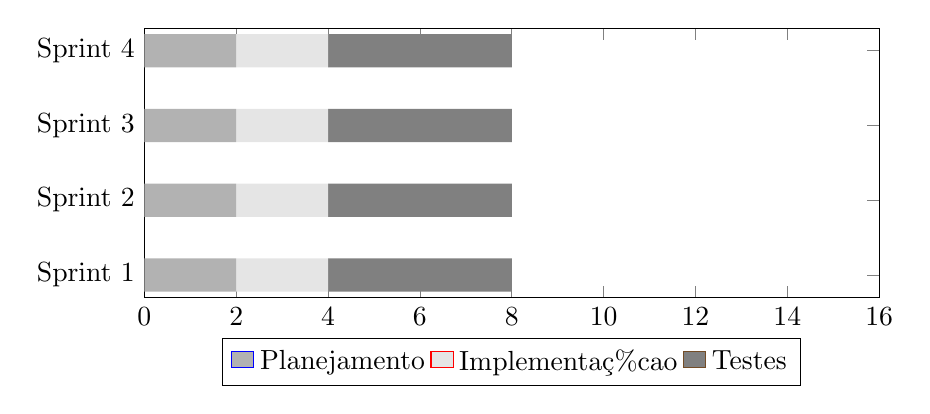
\begin{tikzpicture}
		\begin{axis}[
			xbar stacked,
			xmin=0, xmax=16,
			ytick={1,2,3,4},
			yticklabels={Sprint 1, Sprint 2, Sprint 3, Sprint 4},
			xlabel={Semanas},
			width=0.9\textwidth,
			height=5cm,
			bar width=12pt,
			legend style={at={(0.5,-0.15)},anchor=north,legend columns=3}
			]
			\addplot+[draw=none,fill=black!30] coordinates {(2,4) (2,3) (2,2) (2,1)};
			\addplot+[draw=none,fill=black!10] coordinates {(2,4) (2,3) (2,2) (2,1)};
			\addplot+[draw=none,fill=black!50] coordinates {(4,4) (4,3) (4,2) (4,1)};
			\legend{Planejamento, Implementa\c{c}\%c{a}o, Testes}
		\end{axis}
	\end{tikzpicture}
	\caption{Cronograma simplificado por sprints (exemplo). Ajuste valores conforme seu calend\'ario.}
\end{figure}
% ======= FIM =======


\section*{Template: Issue}

\begin{verbatim}
	# Descri\c{c}\%c{a}o
	# Tarefas
	# Crit\'erios de Aceita\c{c}\%c{a}o
\end{verbatim}
    \chapter{Apêndice C — Roteiro de Aula, Plano de Sprints e Checklist do Semestre}

Este apêndice fornece materiais diretamente aplicáveis em sala de aula, permitindo
que o professor gerencie de forma clara as 16 semanas (4 meses) de trabalho.

%%%%%%%%%%%%%%%%%%%%%%%%%%%%%%%%%%%%%%%%%%%%%%%%%%%%%%%%%%%%%%%%%%%%
\section*{1. Roteiro de Aula Completo (16 Semanas)}

\begin{enumerate}
	\item \textbf{Semana 1:} Apresentação do projeto, formação dos grupos,
	introdução a \ac{git} e estrutura do repositório.
	\item \textbf{Semana 2:} Levantamento de requisitos e primeira modelagem.
	\item \textbf{Semana 3:} Protótipo inicial de telas e arquitetura preliminar.
	\item \textbf{Semana 4:} Definição da \ac{api}, modelo de dados e fluxo geral.
	\item \textbf{Semana 5:} Início da implementação do \gls{backend}.
	\item \textbf{Semana 6:} Início do \gls{frontend} e integração inicial.
	\item \textbf{Semana 7:} Testes manuais e primeira revisão de código.
	\item \textbf{Semana 8:} Construção do \ac{mvp}.
	\item \textbf{Semana 9:} Segunda rodada de testes e refatoração.
	\item \textbf{Semana 10:} Implementação de funcionalidades complementares.
	\item \textbf{Semana 11:} Verificação de segurança e validações.
	\item \textbf{Semana 12:} Testes em fluxo completo (end-to-end).
	\item \textbf{Semana 13:} Documentação técnica e manual do usuário.
	\item \textbf{Semana 14:} Preparação da demo e ensaio.
	\item \textbf{Semana 15:} Entrega final e apresentação pública.
	\item \textbf{Semana 16:} Avaliação pós-projeto e reflexão da equipe.
\end{enumerate}

%%%%%%%%%%%%%%%%%%%%%%%%%%%%%%%%%%%%%%%%%%%%%%%%%%%%%%%%%%%%%%%%%%%%
\section*{2. Plano de Sprints (modelo pronto)}

Cada sprint dura 1 semana.

\subsection*{Sprint 1 — Organização}
	\begin{itemize}
			\item criar repositório;
			\item definir papéis do time;
			\item preparar ambiente;
			\item registrar primeiras \glspl{issue}.
	\end{itemize}

\subsection*{Sprint 2 — Requisitos}
	\begin{itemize}
			\item \glspl{userstory};
			\item restrições;
			\item protótipo simples das telas.
	\end{itemize}

\subsection*{Sprint 3 — Arquitetura}
	\begin{itemize}
			\item fluxos principais;
			\item modelo de dados;
			\item esquema da \ac{api}.
	\end{itemize}

\subsection*{Sprint 4 — \ac{mvp} \gls{backend}}
	\begin{itemize}
			\item rota principal;
			\item validações mínimas;
			\item testes iniciais.
	\end{itemize}

\subsection*{Sprint 5 — \ac{mvp} \gls{frontend}}
	\begin{itemize}
			\item telas funcionais;
			\item integração inicial;
			\item captura de erros.
	\end{itemize}

\subsection*{Sprint 6 — Refinamento}
	\begin{itemize}
			\item refatoração;
			\item revisão de código;
			\item correção de \glspl{bug}.
	\end{itemize}

\subsection*{Sprint 7 — Qualidade}
	\begin{itemize}
			\item testes completos;
			\item revisão da \ac{api};
			\item estabilização.
	\end{itemize}

\subsection*{Sprint 8 — Entrega Final}
	\begin{itemize}
			\item documentação;
			\item preparação da apresentação;
			\item \gls{release} final.
			\item (Opcional) Material para o professor.
	\end{itemize}

%%%%%%%%%%%%%%%%%%%%%%%%%%%%%%%%%%%%%%%%%%%%%%%%%%%%%%%%%%%%%%%%%%%%
\section*{3. Checklist Geral do Semestre}

\subsection*{Checklist Técnico}
	\begin{itemize}
			\item requisitos claros e documentados;
			\item arquitetura desenhada;
			\item \ac{api} definida e testada;
			\item banco de dados funcional;
			\item interface completa;
			\item validações implementadas;
			\item testes documentados;
			\item \glspl{bug} críticos resolvidos;
			\item manual de usuário pronto;
			\item \gls{release} final disponível.
	\end{itemize}

\subsection*{Checklist de Equipe}
	\begin{itemize}
			\item papéis definidos;
			\item reuniões semanais realizadas;
			\item \glspl{issue} abertas e fechadas regularmente;
			\item comunicação clara no repositório;
			\item revisão de código aplicada;
			\item conflitos resolvidos rapidamente.
	\end{itemize}

\subsection*{Checklist de Apresentação}
	\begin{itemize}
			\item roteiro claro;
			\item tempo ensaiado;
			\item demo pronta e testada;
			\item prints como plano B;
			\item domínio do sistema;
			\item divisão equilibrada das falas.
	\end{itemize}

%%%%%%%%%%%%%%%%%%%%%%%%%%%%%%%%%%%%%%%%%%%%%%%%%%%%%%%%%%%%%%%%%%%%
\section*{4. Material Extra para o Professor}

Sugestões práticas:

	\begin{itemize}
			\item usar rubricas de avaliação semanais;
			\item criar painéis visuais de progresso;
			\item promover sessões rápidas de mentoria por grupo;
			\item incentivar alunos a registrar microvitórias;
			\item intercalar teoria e prática a cada aula.
	\end{itemize}

%%%%%%%%%%%%%%%%%%%%%%%%%%%%%%%%%%%%%%%%%%%%%%%%%%%%%%%%%%%%%%%%%%%%
\section*{5. Encerramento do Apêndice}

Este apêndice fornece um conjunto completo de ferramentas operacionais para
organizar, conduzir e avaliar o projeto ao longo de quatro meses, garantindo
clareza, estrutura, ritmo e coerência pedagógica.

\section*{Template: Pull Request}

\begin{verbatim}
	# O que foi feito
	# Como testar
	# Checklist
\end{verbatim}


\end{document}